\documentclass[./main.tex]{subfiles}

\begin{document}
\section{Dataset}
\ref{sec:dataset}
To perform the pose estimation in Section \ref{sec:experiments}, we need some data on which to train, validate and test our models. The following section describes the datasets that will be used. This starts off in section \ref{sec:ClimbAlong}, where we describe the dataset provided by ClimbAlong. This is then followed by section \ref{sec:BRACE} and section \ref{sec:PA}, where we describe the datasets that we will be used during pretraining of our models.

\begin{table}[htbp]
    \begin{tabular}{|l|c|c|c|c|}
        \hline
        \textbf{Keypoint label} & \textbf{ClimbAlong} & \textbf{BRACE} & \textbf{Penn Action} \\ \hline
        Head & No & No & Yes \\ \hline
        Nose & Yes & Yes & No \\ \hline
        Left ear & Yes & Yes & No \\ \hline
        Right ear & Yes & Yes & No \\ \hline
        Left eye & No & Yes & No \\ \hline
        Right eye & No & Yes & No \\ \hline
        Left shoulder & Yes & Yes & Yes \\ \hline
        Right shoulder & Yes & Yes & Yes \\ \hline
        Left elbow & Yes & Yes & Yes \\ \hline
        Right elbow & Yes & Yes & Yes \\ \hline
        Left wrist & Yes & Yes & Yes \\ \hline
        Right wrist & Yes & Yes & Yes \\ \hline
        Left pinky & Yes & No & No \\ \hline
        Right pinky & Yes & No & No \\ \hline
        Left index & Yes & No & No \\ \hline
        Right index & Yes & No & No \\ \hline
        Left thumb & Yes & No & No \\ \hline
        Right thumb & Yes & No & No \\ \hline
        Left hip & Yes & Yes & Yes \\ \hline
        Right hip & Yes & Yes & Yes \\ \hline
        Left knee & Yes & Yes & Yes \\ \hline
        Right knee & Yes & Yes & Yes \\ \hline
        Left ankle & Yes & Yes & Yes \\ \hline
        Right ankle & Yes & Yes & Yes \\ \hline
        Left heel & Yes & No & No \\ \hline
        Right heel & Yes & No & No \\ \hline
        Left toes & Yes & No & No \\ \hline
        Right toes & Yes & No & No \\ \hline
    \end{tabular}
    \caption{Overview of the annotated keypoints of the three used datasets}
    \label{tab:keypoints}
\end{table}

\subsection{The ClimbAlong Dataset}
\label{sec:ClimbAlong}
\begin{figure}[htbp]
    \centering
    \begin{subfigure}{0.3\textwidth}
        \centering
        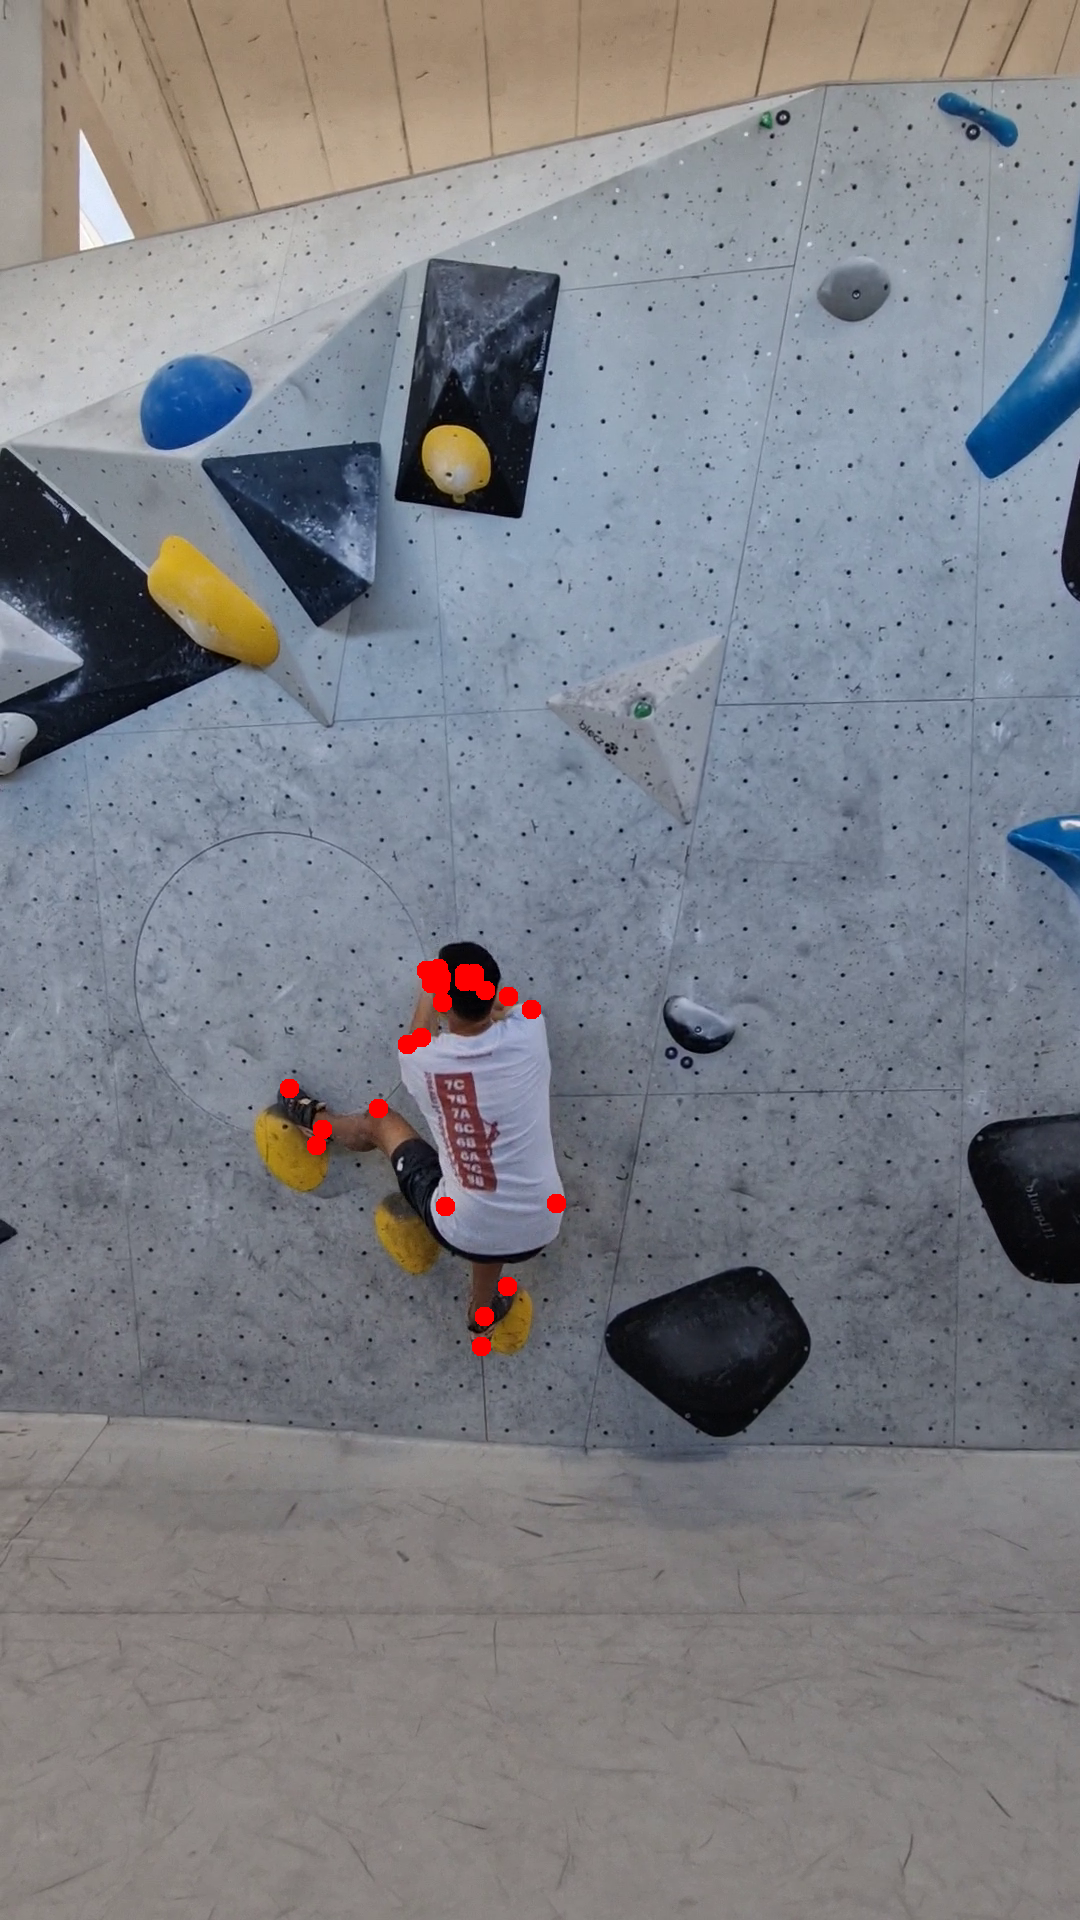
\includegraphics[width=\textwidth]{entities/CA_17.png}
        \caption{Frame 17}
    \end{subfigure}
    \begin{subfigure}{0.3\textwidth}
        \centering
        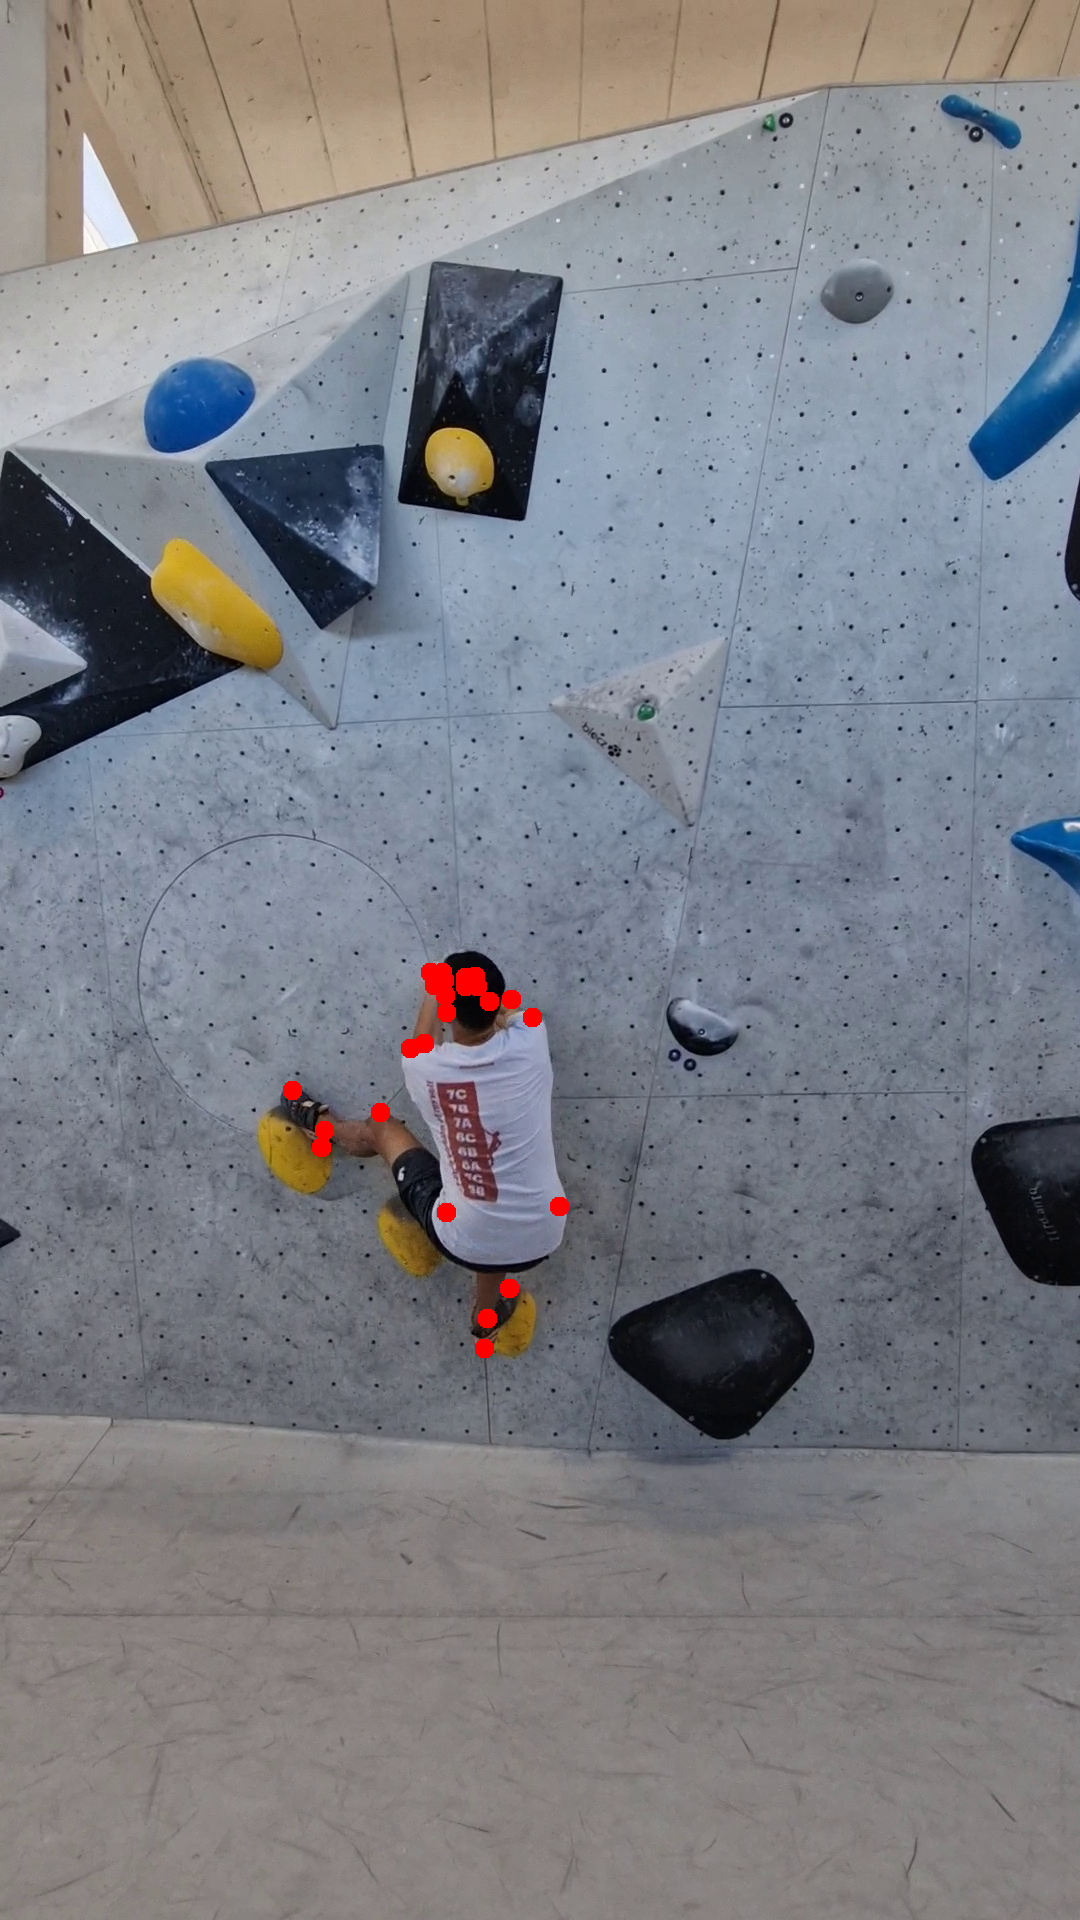
\includegraphics[width=\textwidth]{entities/CA_18.png}
        \caption{Frame 18}
    \end{subfigure}
    \begin{subfigure}{0.3\textwidth}
        \centering
        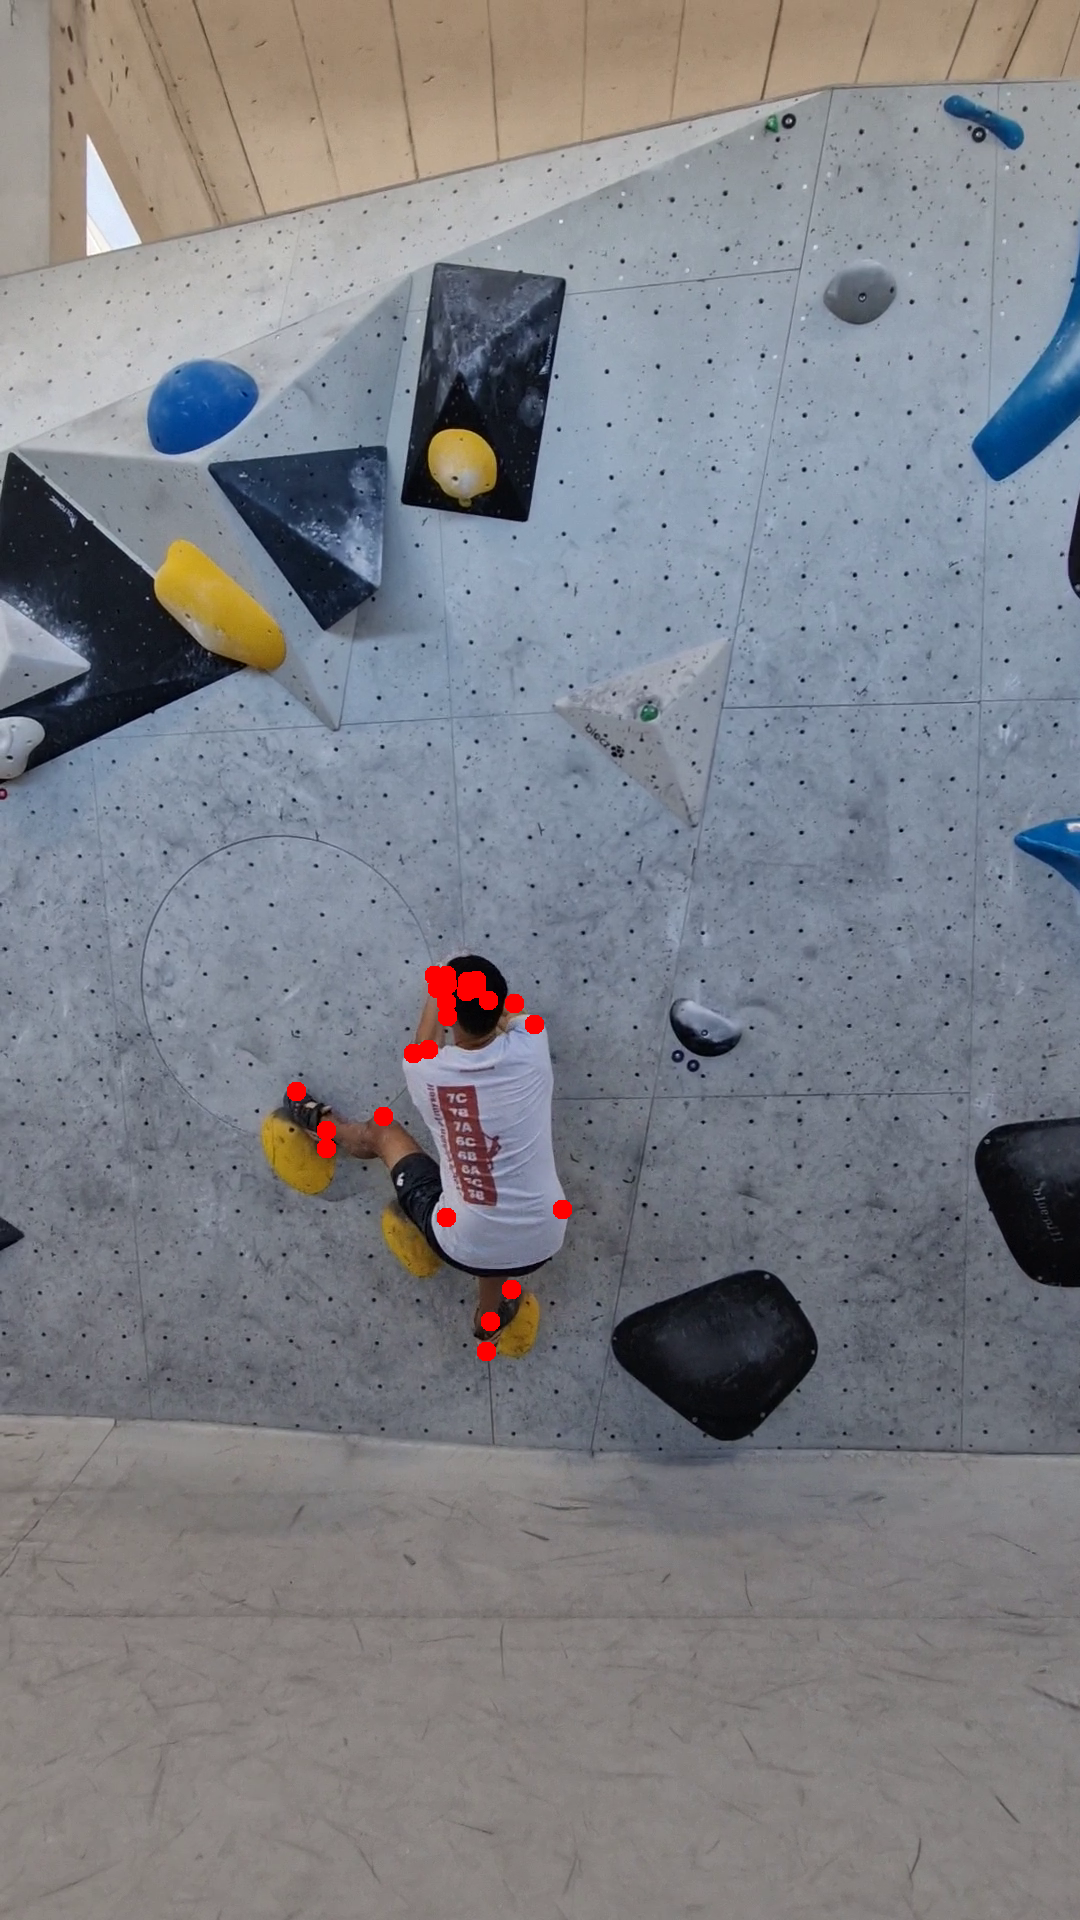
\includegraphics[width=\textwidth]{entities/CA_19.png}
        \caption{Frame 19}
    \end{subfigure}
    \begin{subfigure}{0.3\textwidth}
        \centering
        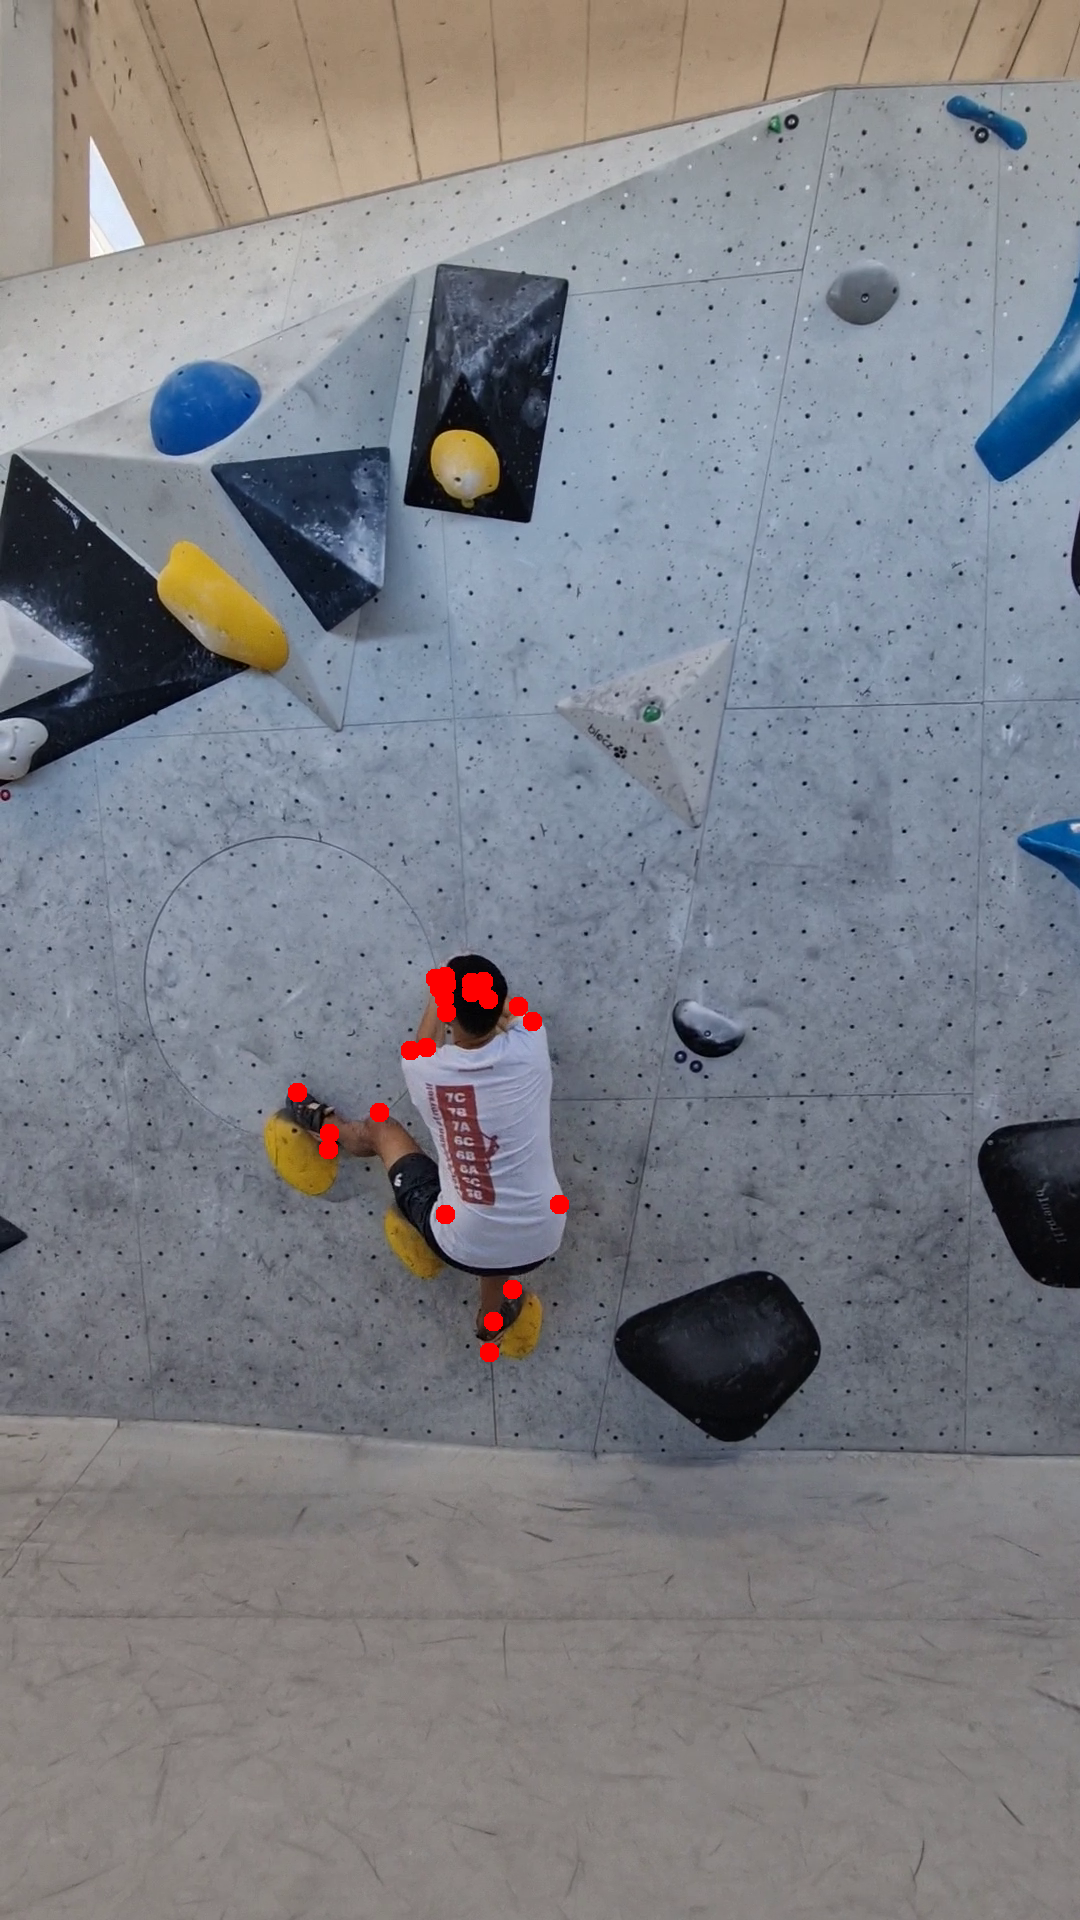
\includegraphics[width=\textwidth]{entities/CA_20.png}
        \caption{Frame 20}
    \end{subfigure}
    \begin{subfigure}{0.3\textwidth}
        \centering
        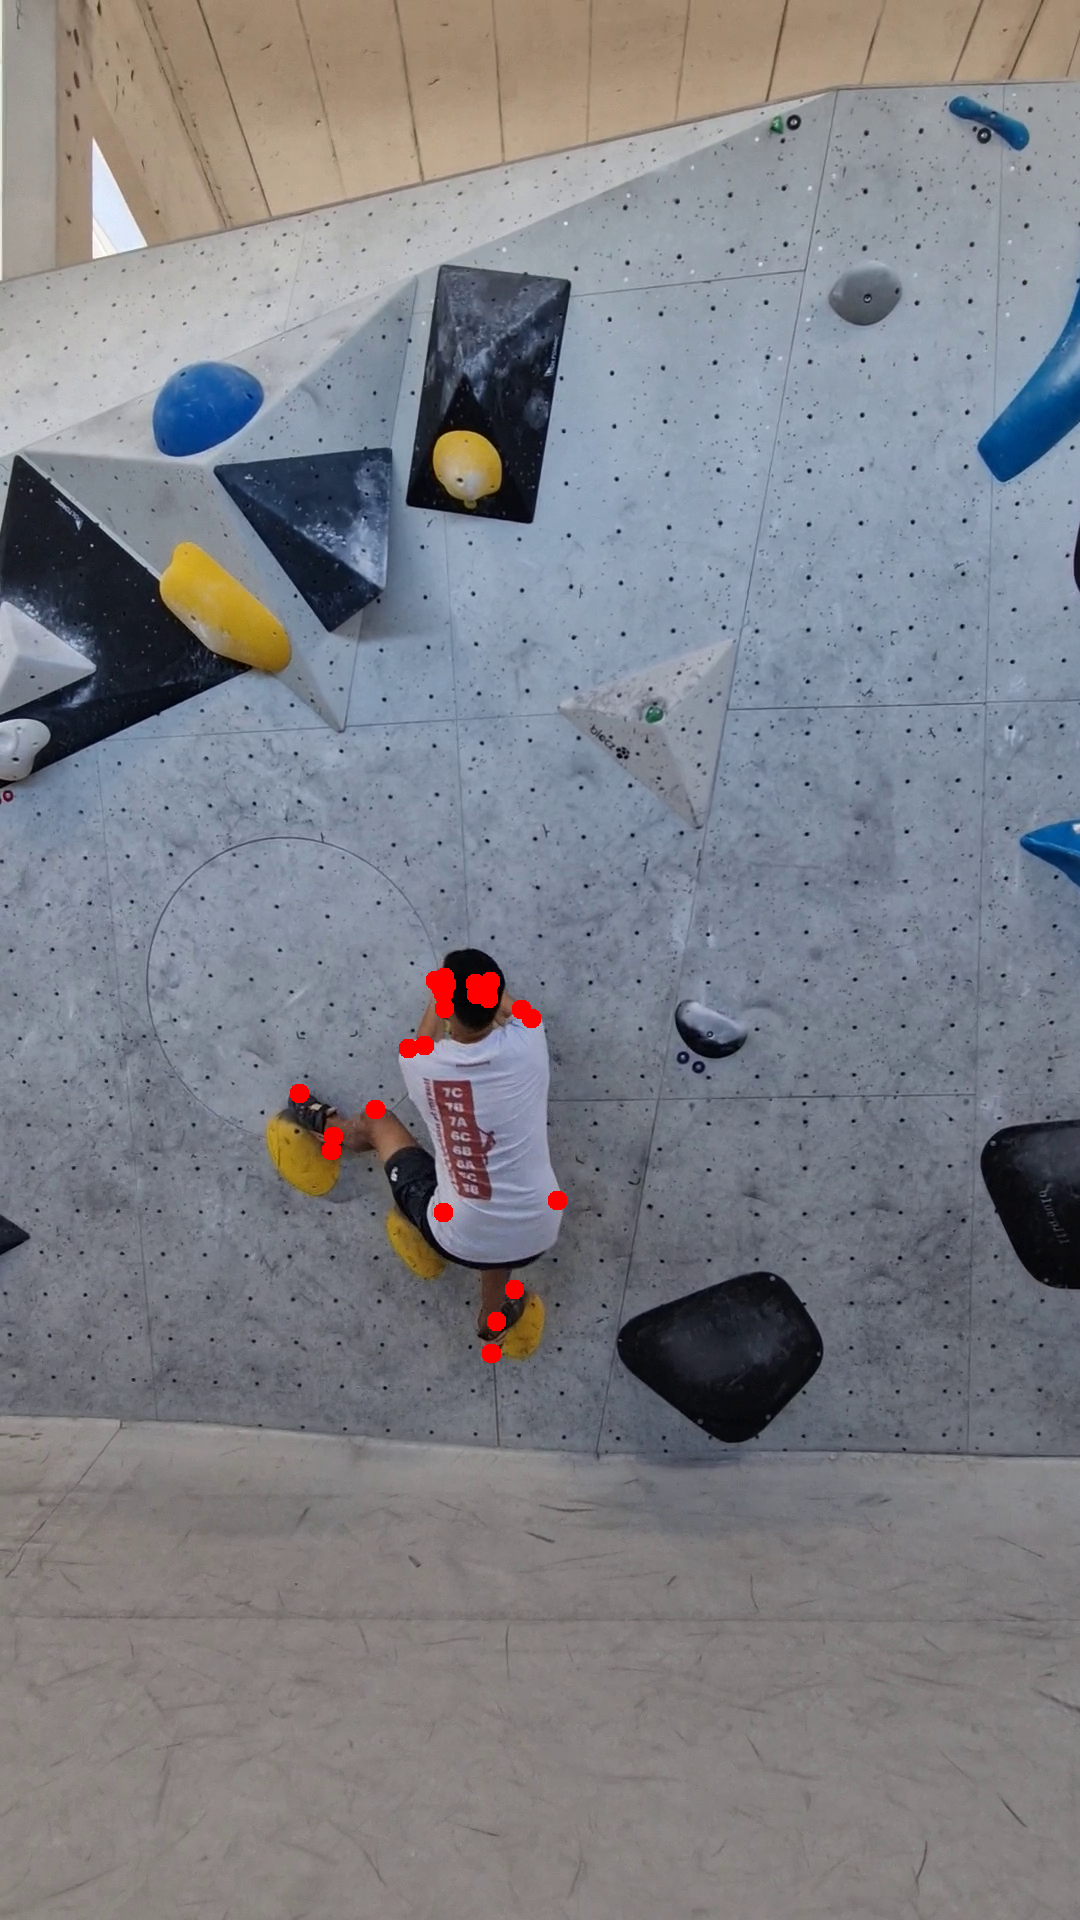
\includegraphics[width=\textwidth]{entities/CA_21.png}
        \caption{Frame 21}
    \end{subfigure}
    \caption{Example of five consecutive frames of a video from the ClimbAlong dataset with the corresponding groundtruth keypoints, where the actor holds his position for a while.}
    \label{fig:CA_dataset_static}
\end{figure}

\begin{figure}[htbp]
    \centering
    \begin{subfigure}{0.3\textwidth}
        \centering
        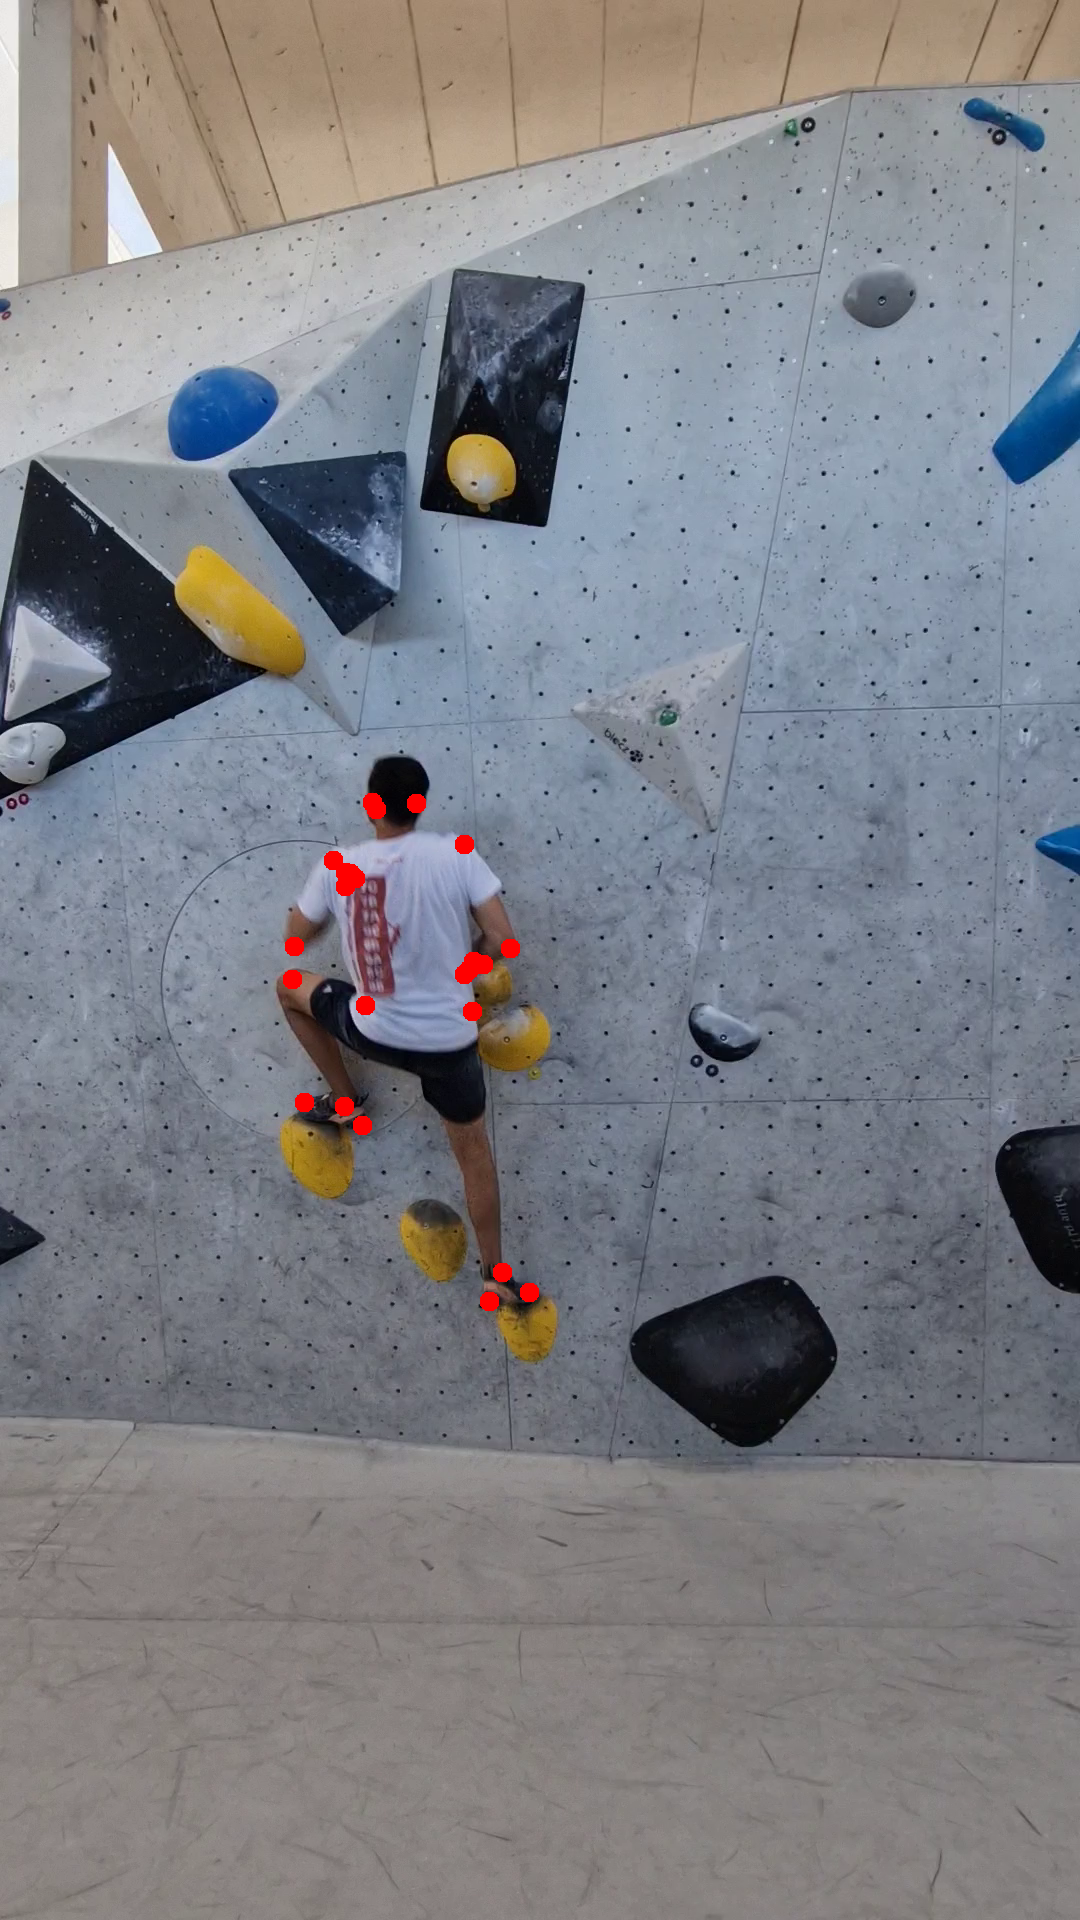
\includegraphics[width=\textwidth]{entities/CA_31.png}
        \caption{Frame 31}
    \end{subfigure}
    \begin{subfigure}{0.3\textwidth}
        \centering
        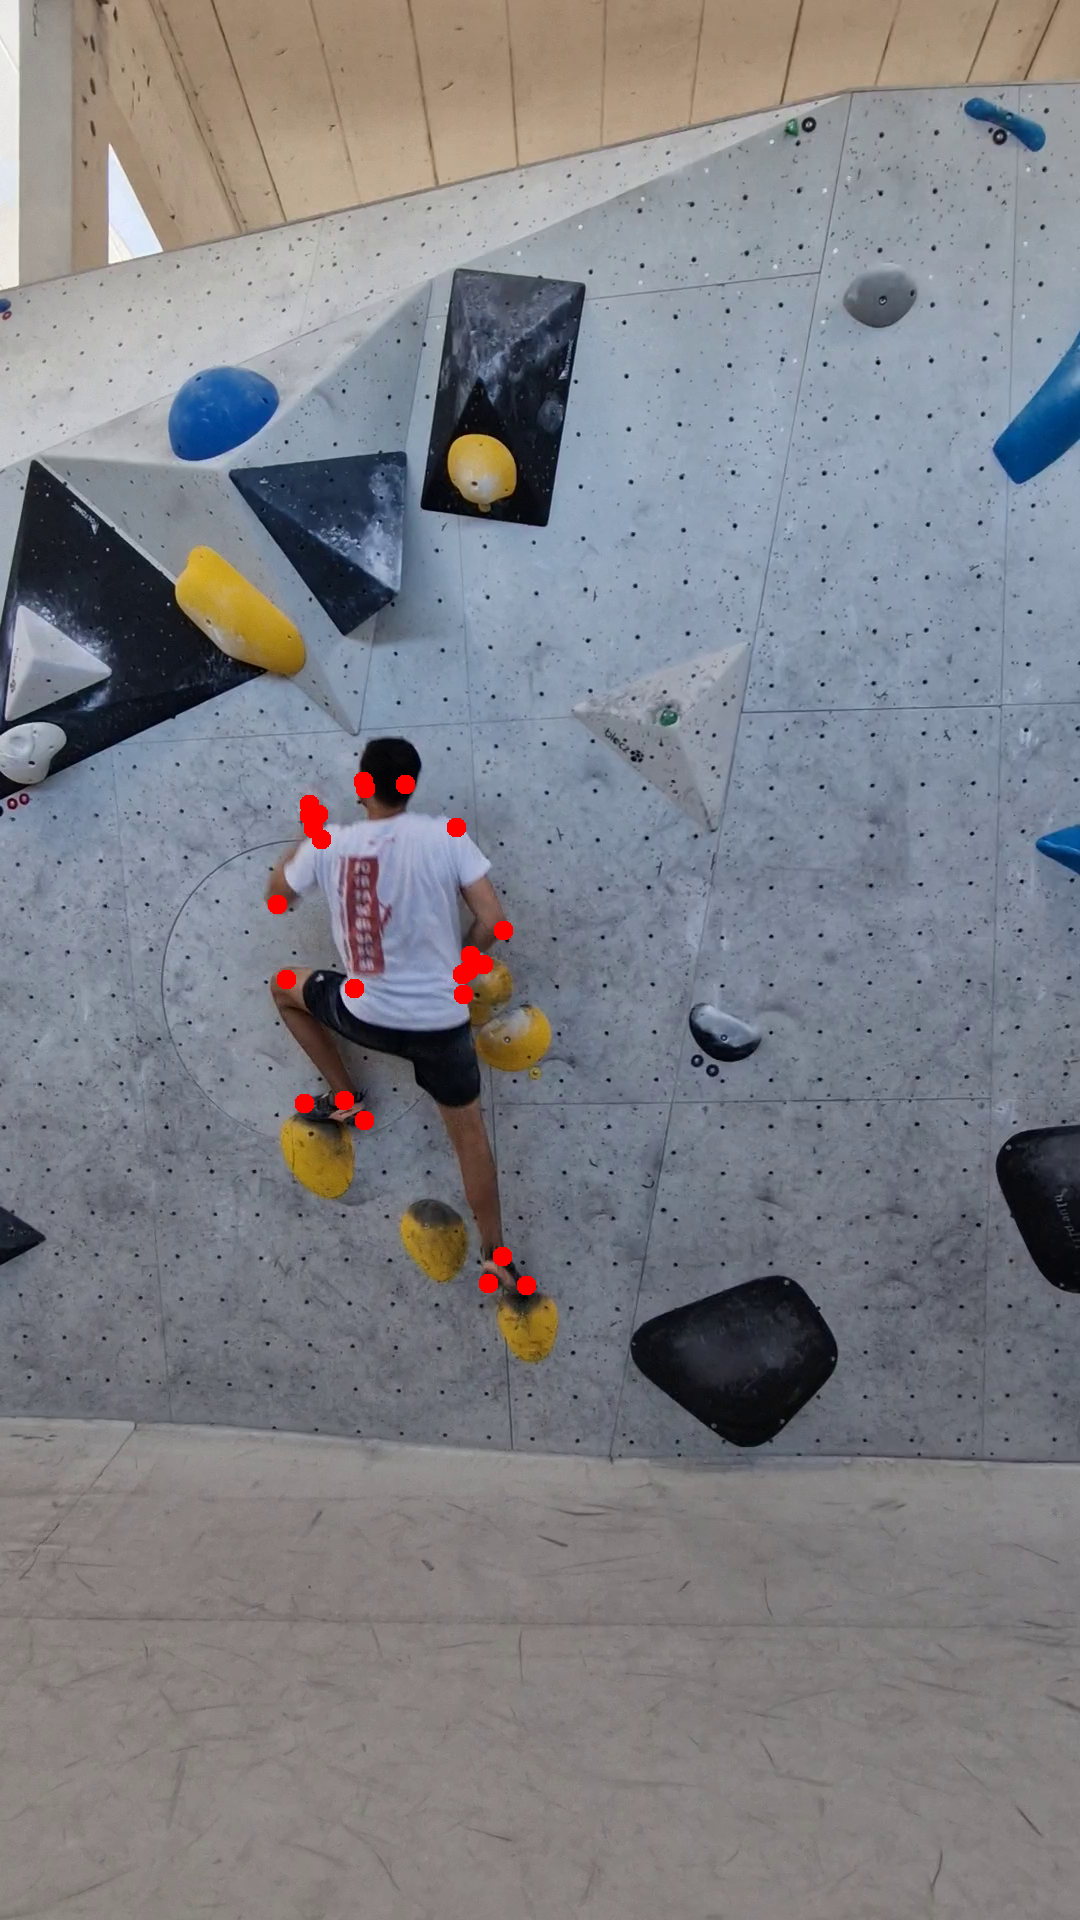
\includegraphics[width=\textwidth]{entities/CA_32.png}
        \caption{Frame 32}
    \end{subfigure}
    \begin{subfigure}{0.3\textwidth}
        \centering
        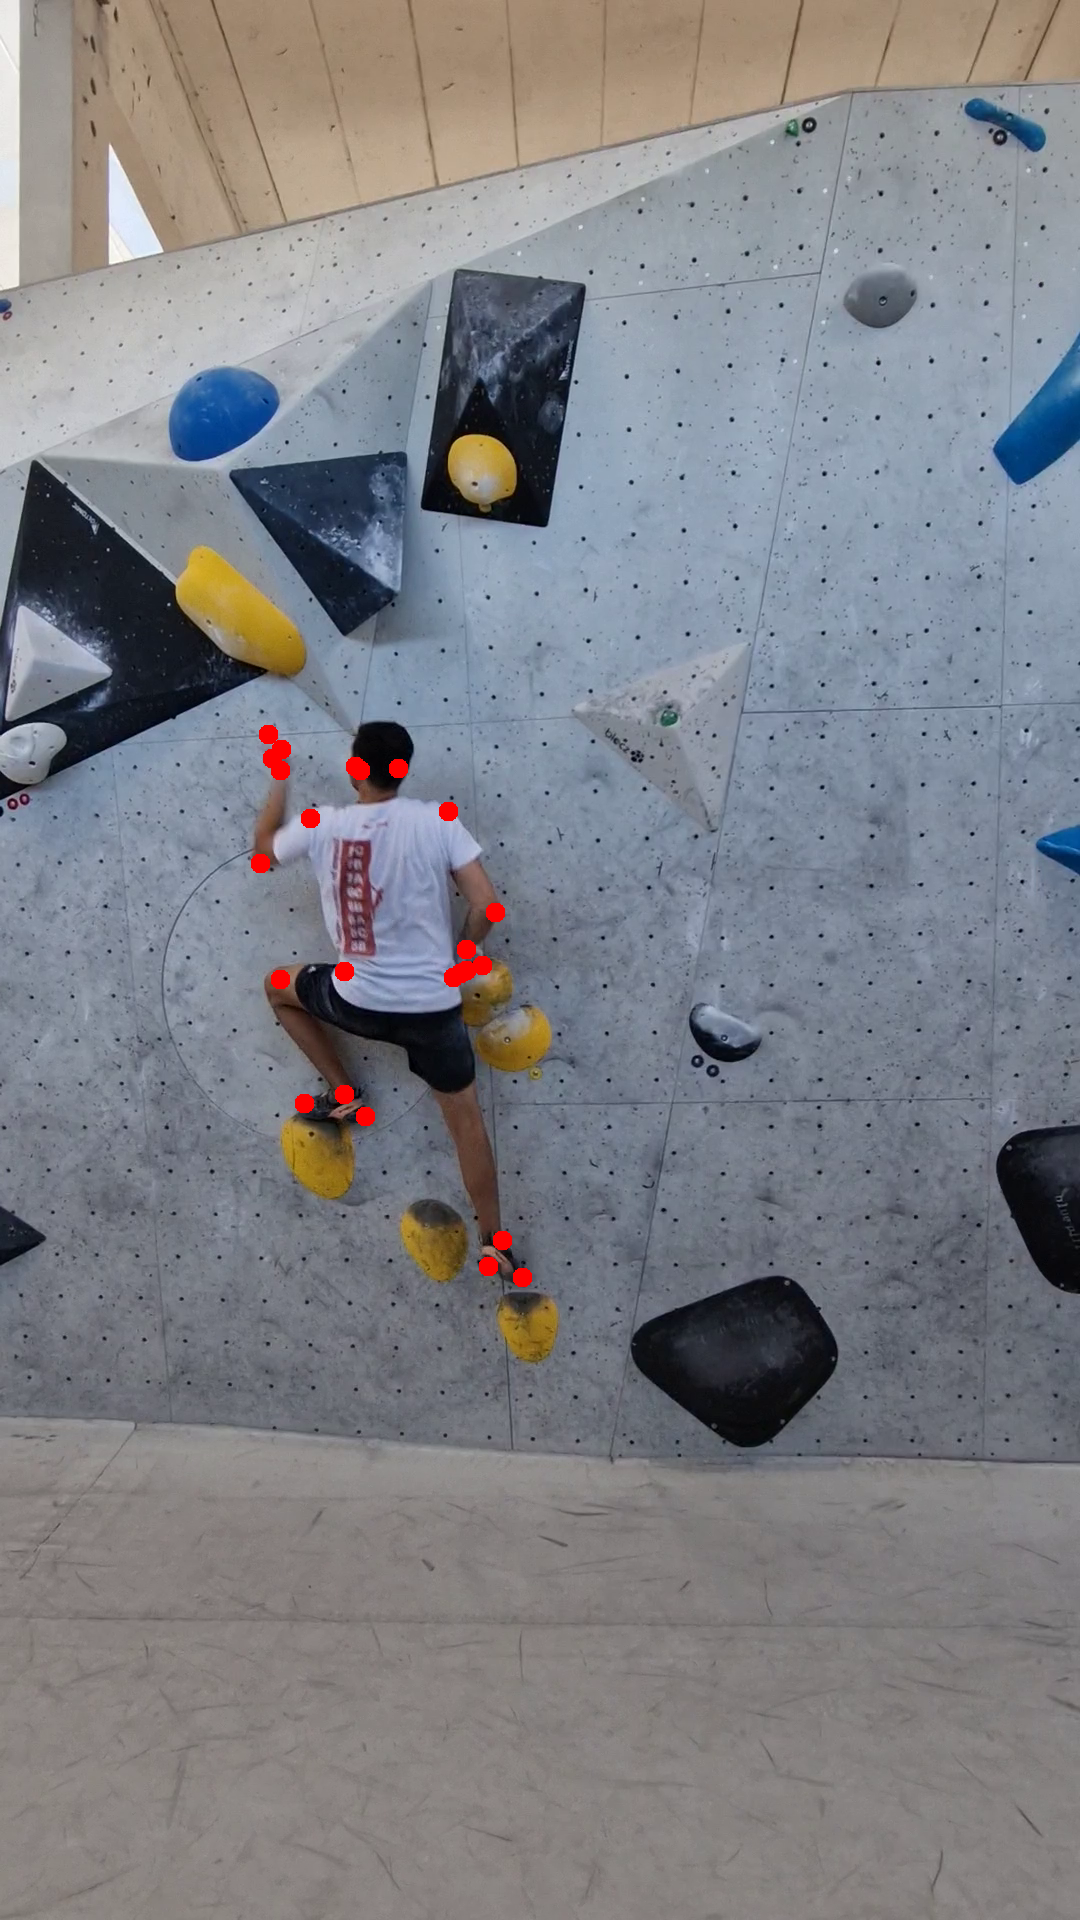
\includegraphics[width=\textwidth]{entities/CA_33.png}
        \caption{Frame 33}
    \end{subfigure}
    \begin{subfigure}{0.3\textwidth}
        \centering
        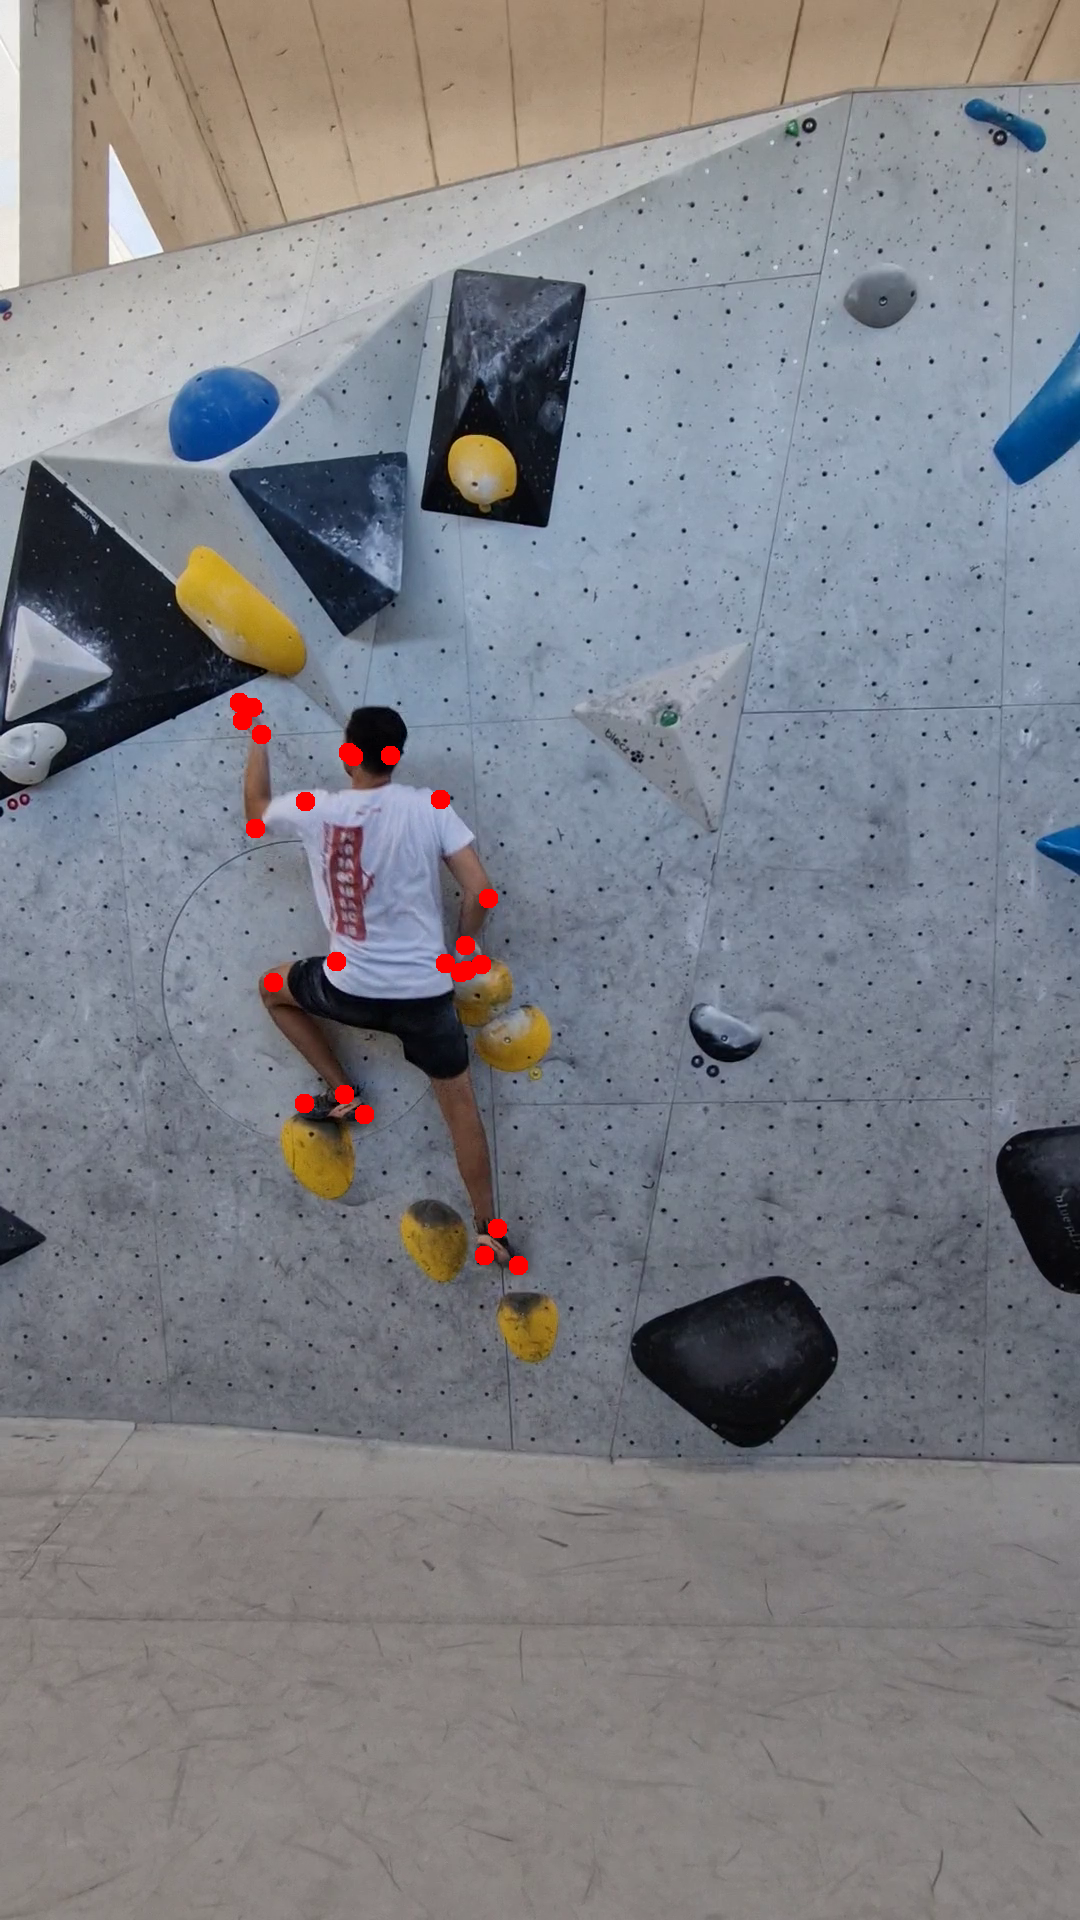
\includegraphics[width=\textwidth]{entities/CA_34.png}
        \caption{Frame 34}
    \end{subfigure}
    \begin{subfigure}{0.3\textwidth}
        \centering
        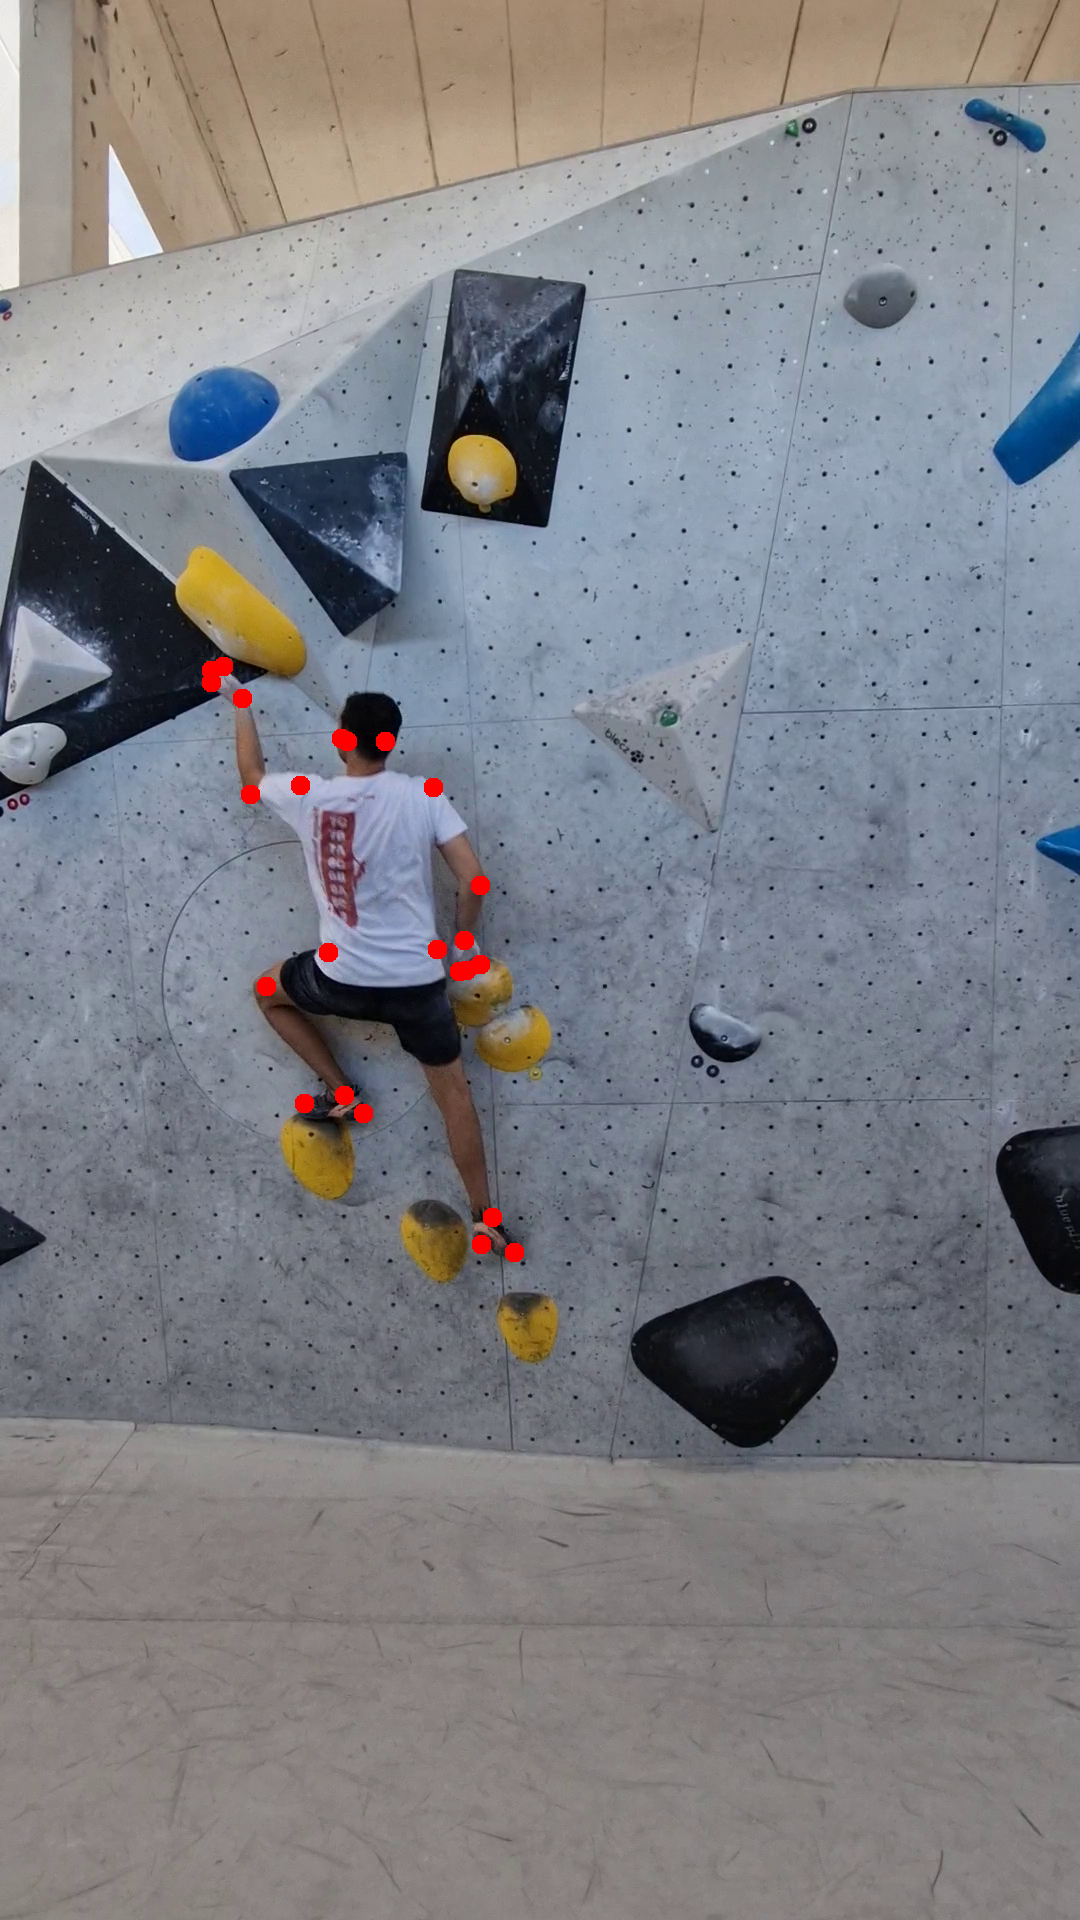
\includegraphics[width=\textwidth]{entities/CA_35.png}
        \caption{Frame 35}
    \end{subfigure}

    \caption{Example of five consecutive frames of a video from the ClimbAlong dataset with the corresponding groundtruth keypoints, where the actor performs a quick movement.}
    \label{fig:CA_dataset_quick}
\end{figure}

As the aim of our models is to perform well on climbers, we will be using some annotated data of climbers. For this, ClimbAlong has developed a dataset that we will be using. The dataset consists of videos of various climbers on bouldering walls, where each video contains just a single climber. Figure \ref{fig:CA_dataset_static} and \ref{fig:CA_dataset_quick} illustrates two windows of five consecutive frames of a single video from the ClimbAlong dataset. As shown in the figures, the videos in the dataset contains both static positions, where the climber holds a position for a while, as well as quick movements.
\\
\\
The dataset consists of $30$ fully annotated videos and a total of $10,293$ fully annotated frames, where each annotation consists of $25$ keypoints. Table \ref{tab:keypoints} gives an overview of which keypoints are annotated in the dataset. Each videos is filmed in portrait mode with a resolution of $1080 \times 1920$ and $30$ frames per second.

\subsection{The BRACE Dataset}
\label{sec:BRACE}
\begin{figure}[htbp]
    \centering
    \begin{subfigure}{0.45\textwidth}
        \centering
        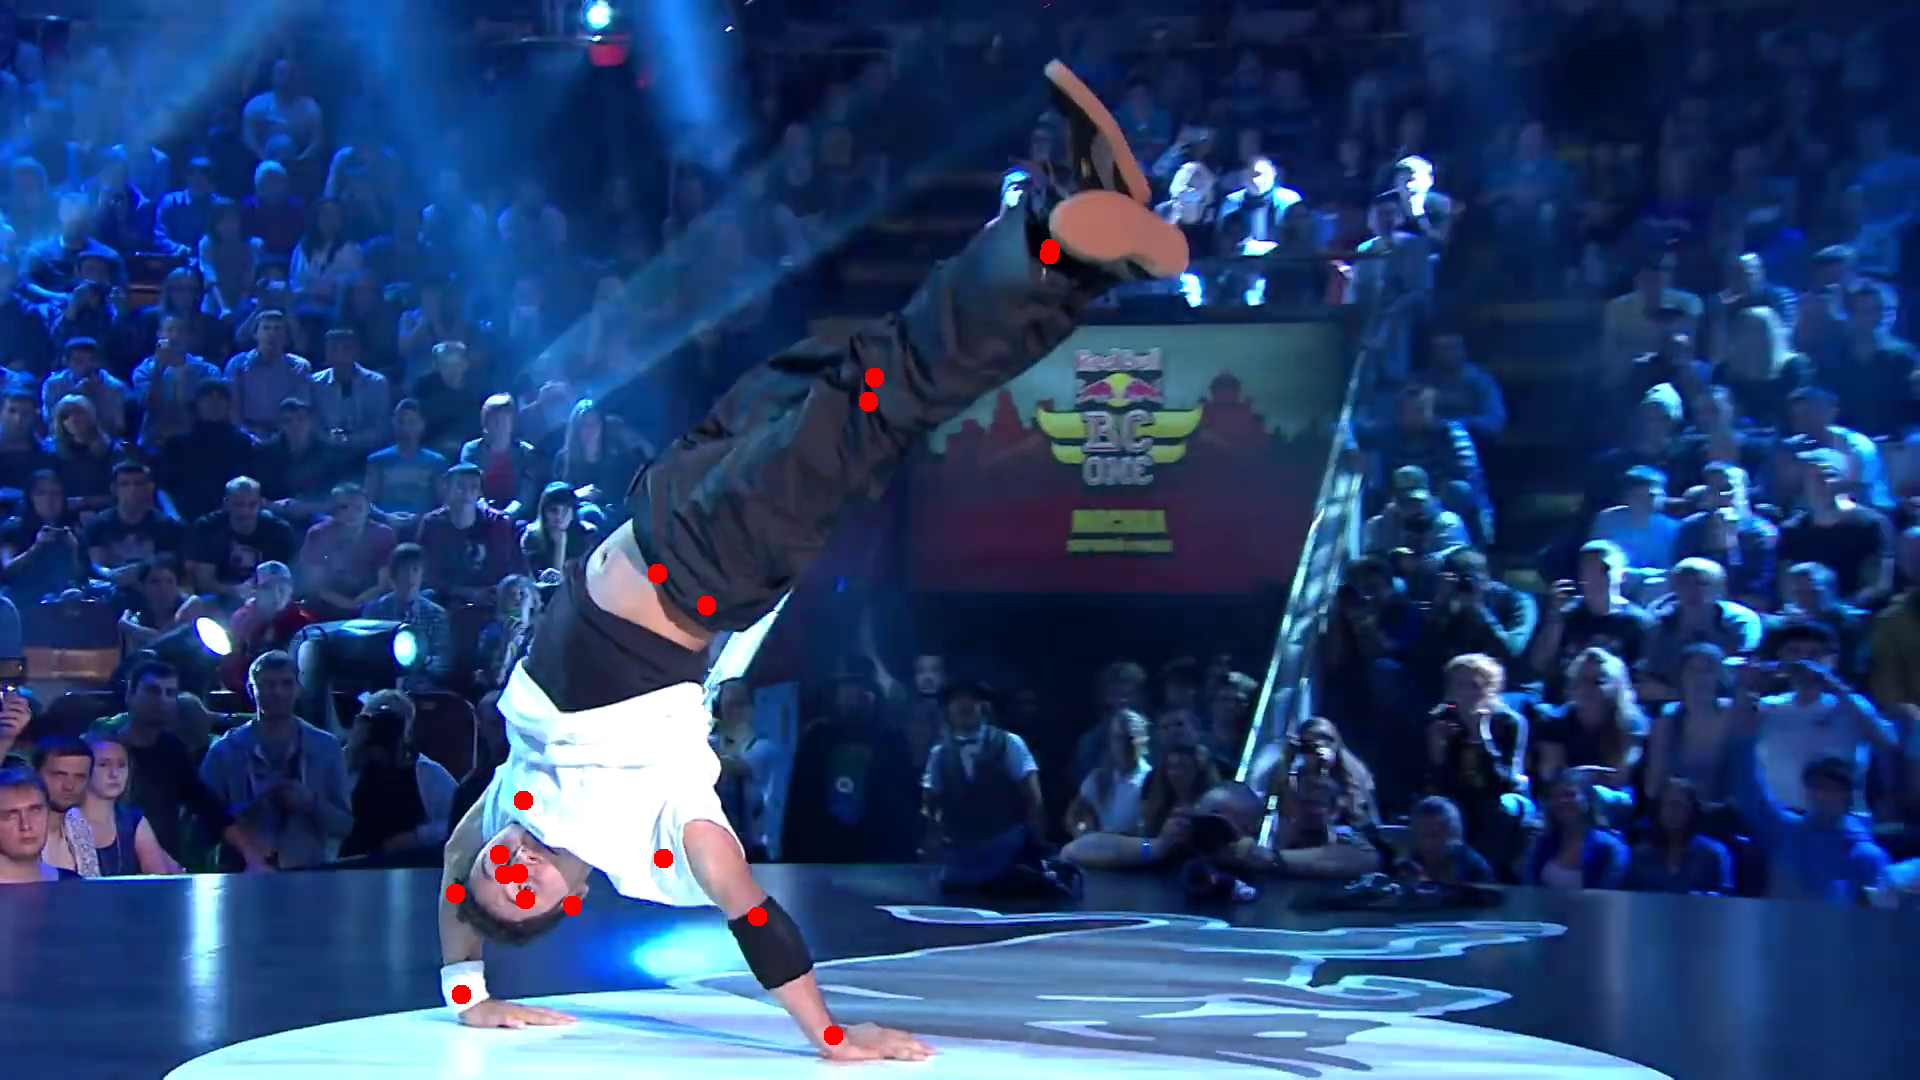
\includegraphics[width=\textwidth]{entities/BRACE_2450.png}
        \caption{Frame 2450}
    \end{subfigure}
    \begin{subfigure}{0.45\textwidth}
        \centering
        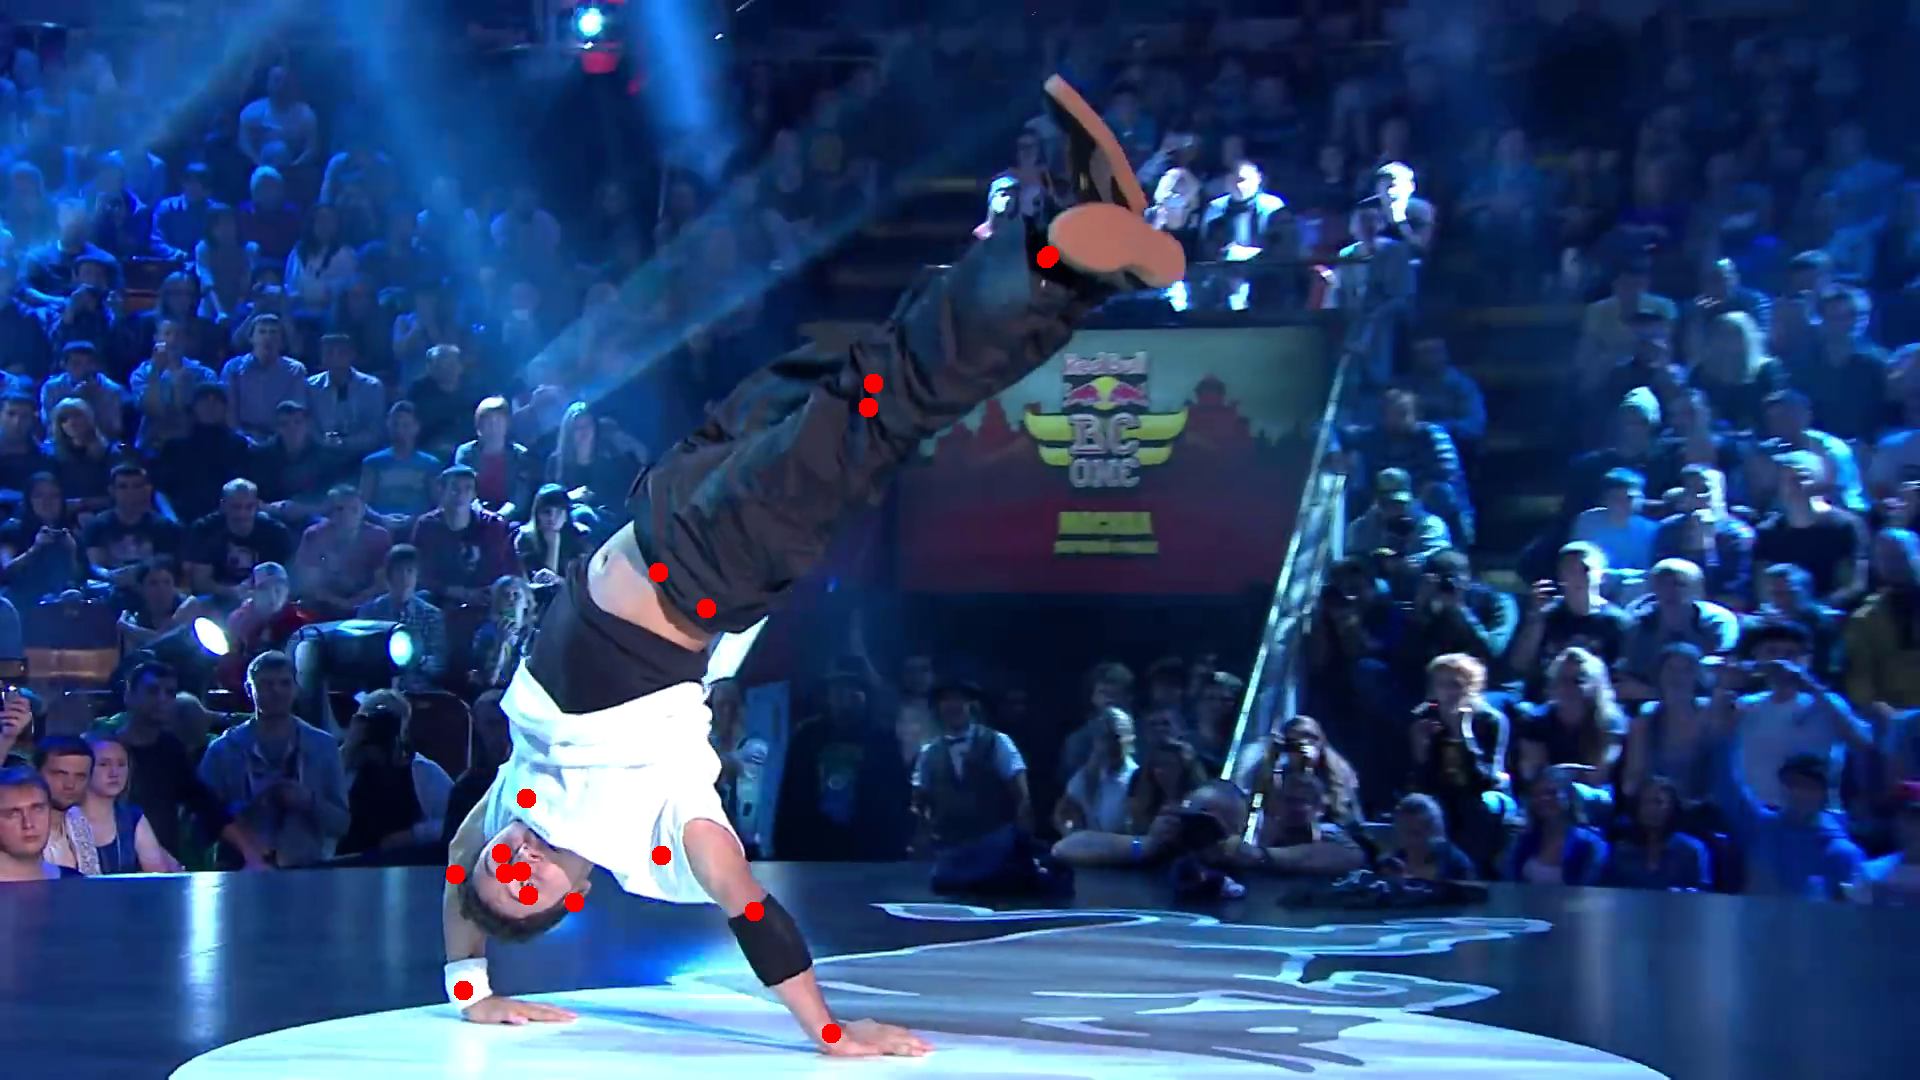
\includegraphics[width=\textwidth]{entities/BRACE_2451.png}
        \caption{Frame 2451}
    \end{subfigure}
    \begin{subfigure}{0.45\textwidth}
        \centering
        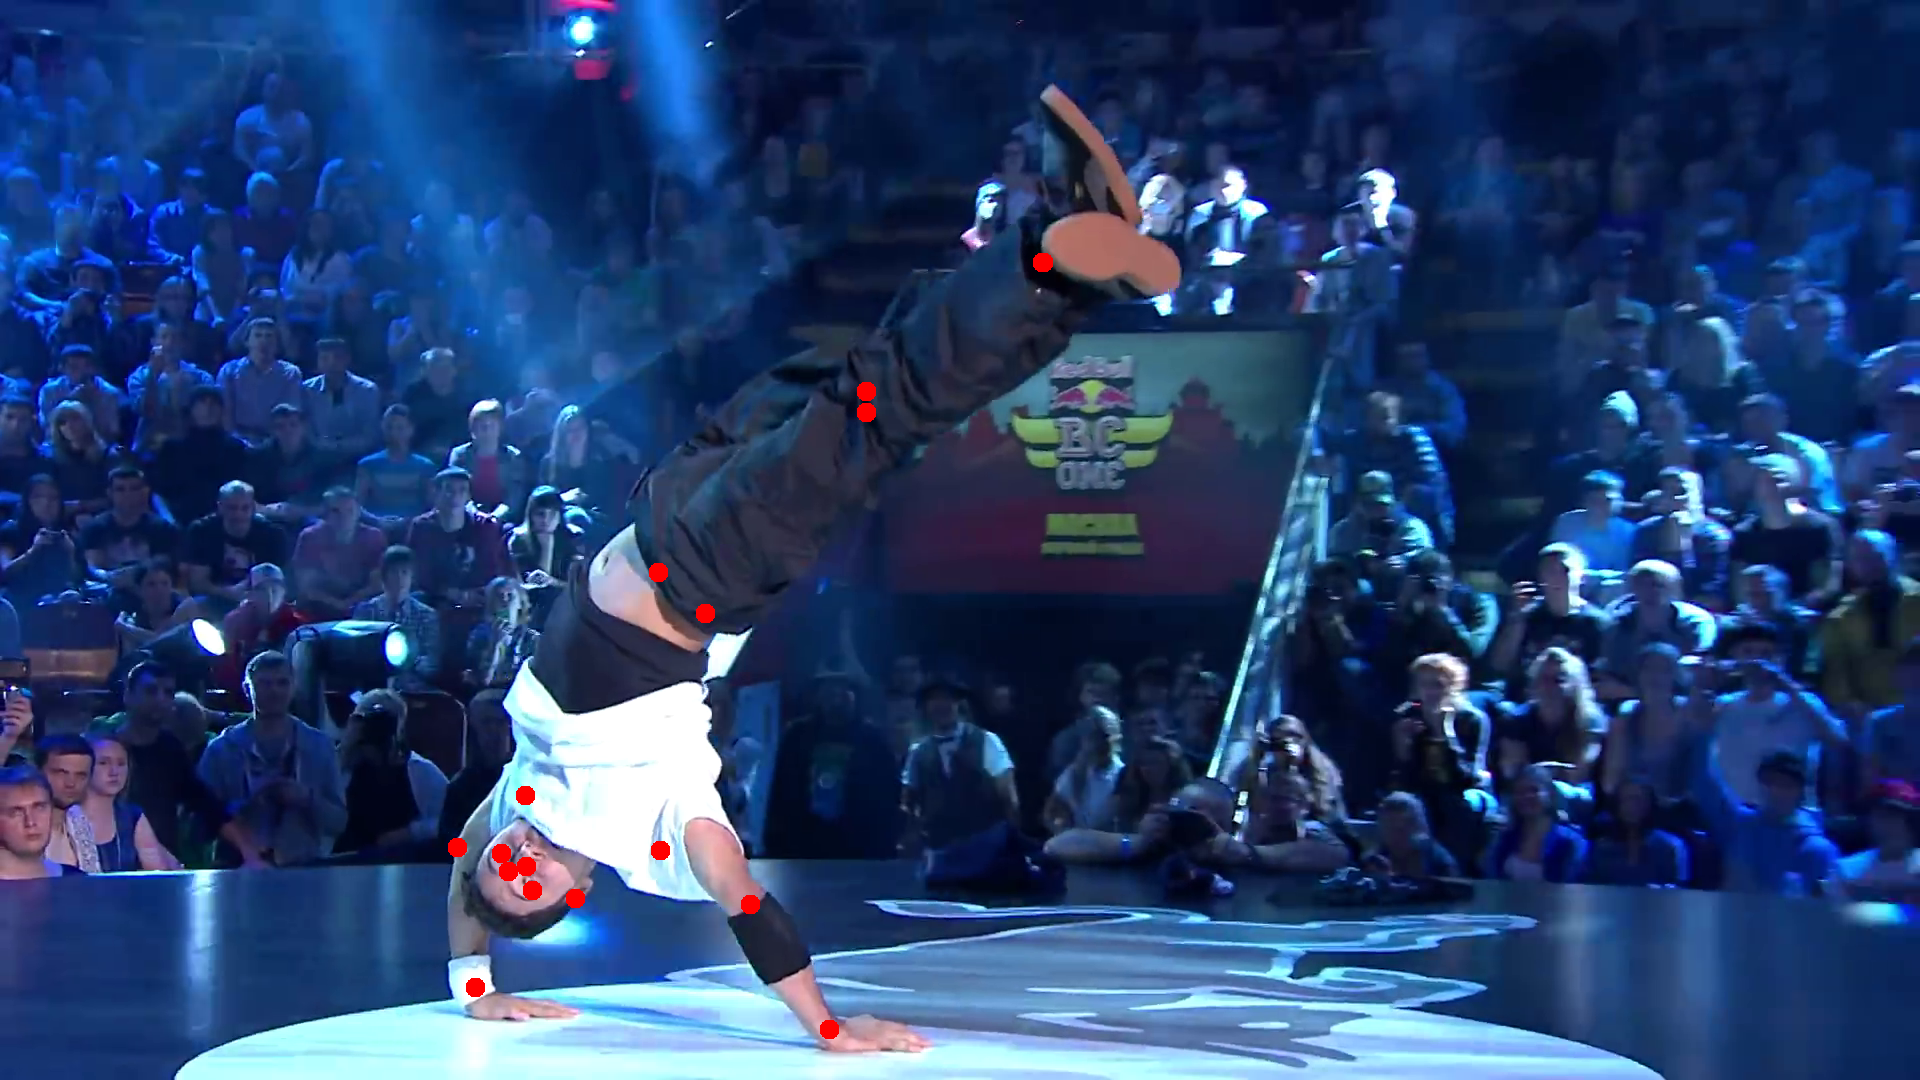
\includegraphics[width=\textwidth]{entities/BRACE_2452.png}
        \caption{Frame 2452}
    \end{subfigure}
    \begin{subfigure}{0.45\textwidth}
        \centering
        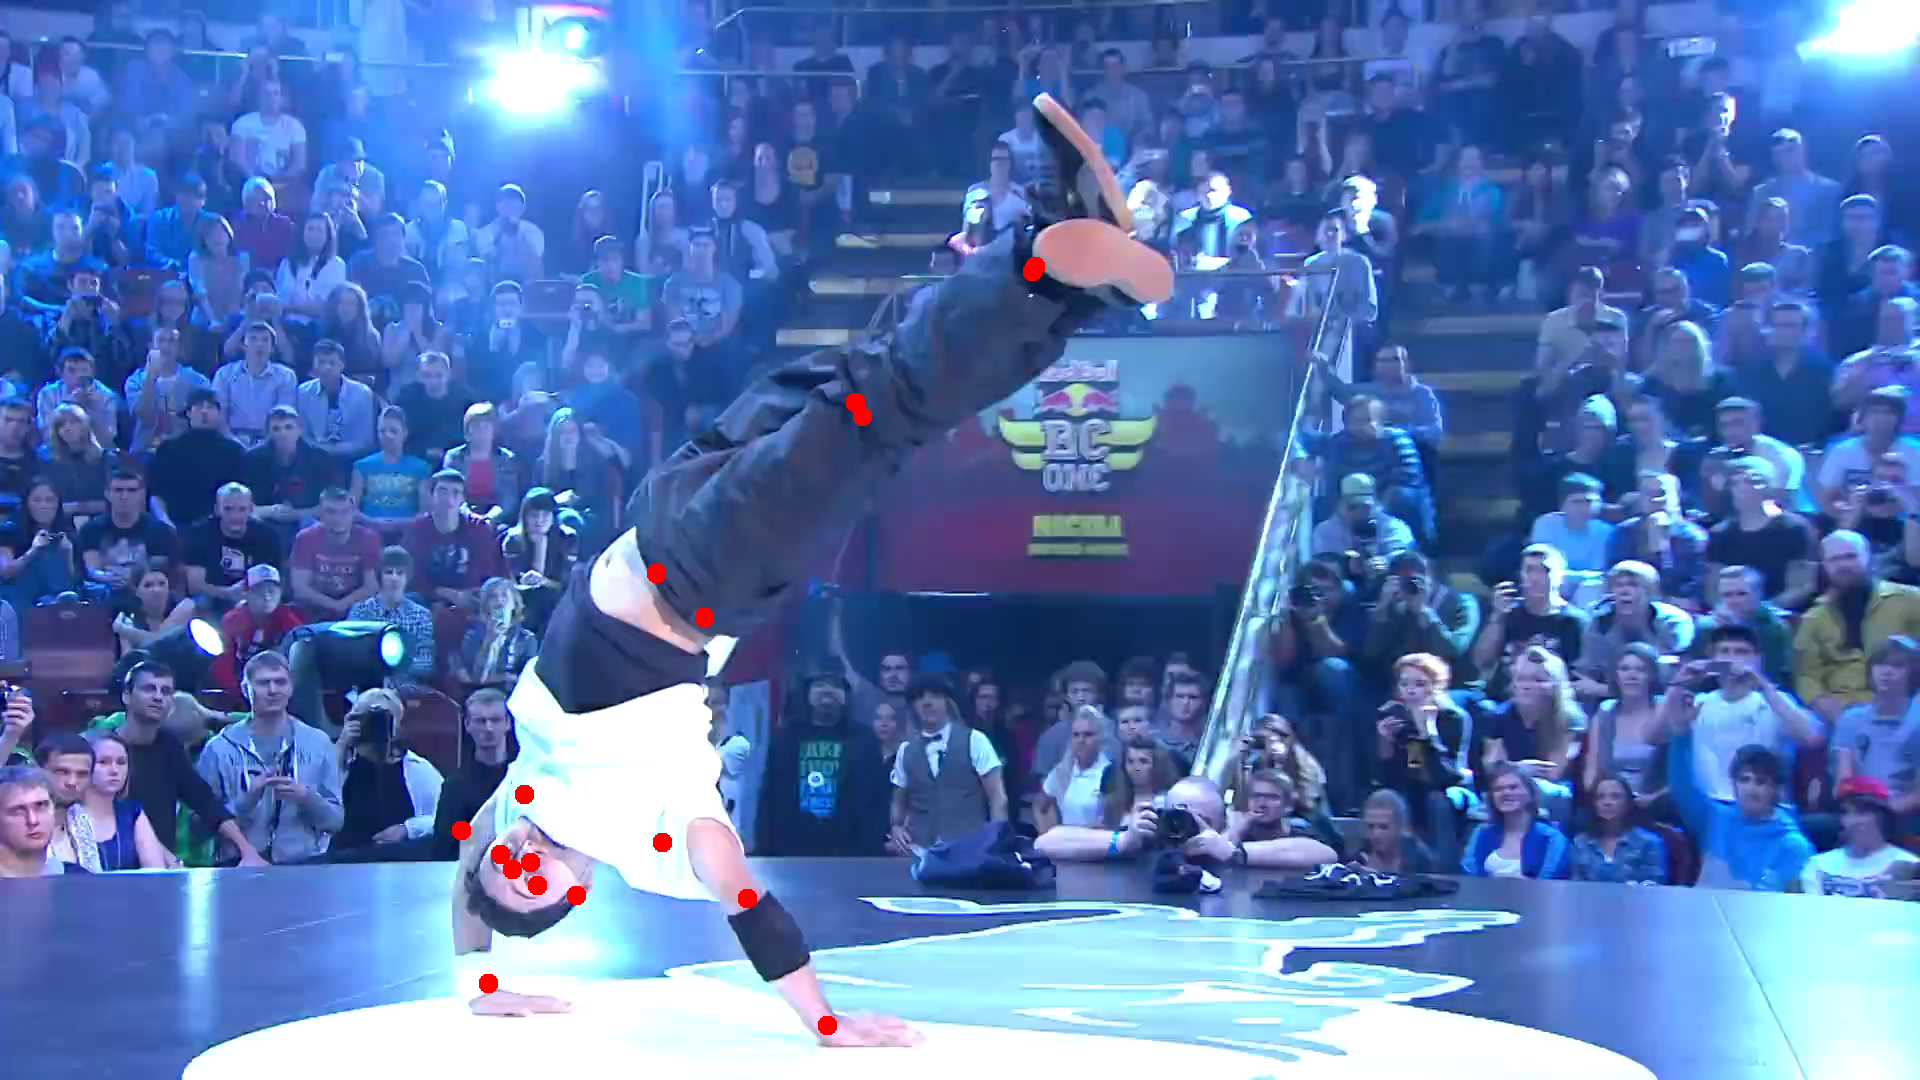
\includegraphics[width=\textwidth]{entities/BRACE_2453.png}
        \caption{Frame 2453}
    \end{subfigure}
    \begin{subfigure}{0.45\textwidth}
        \centering
        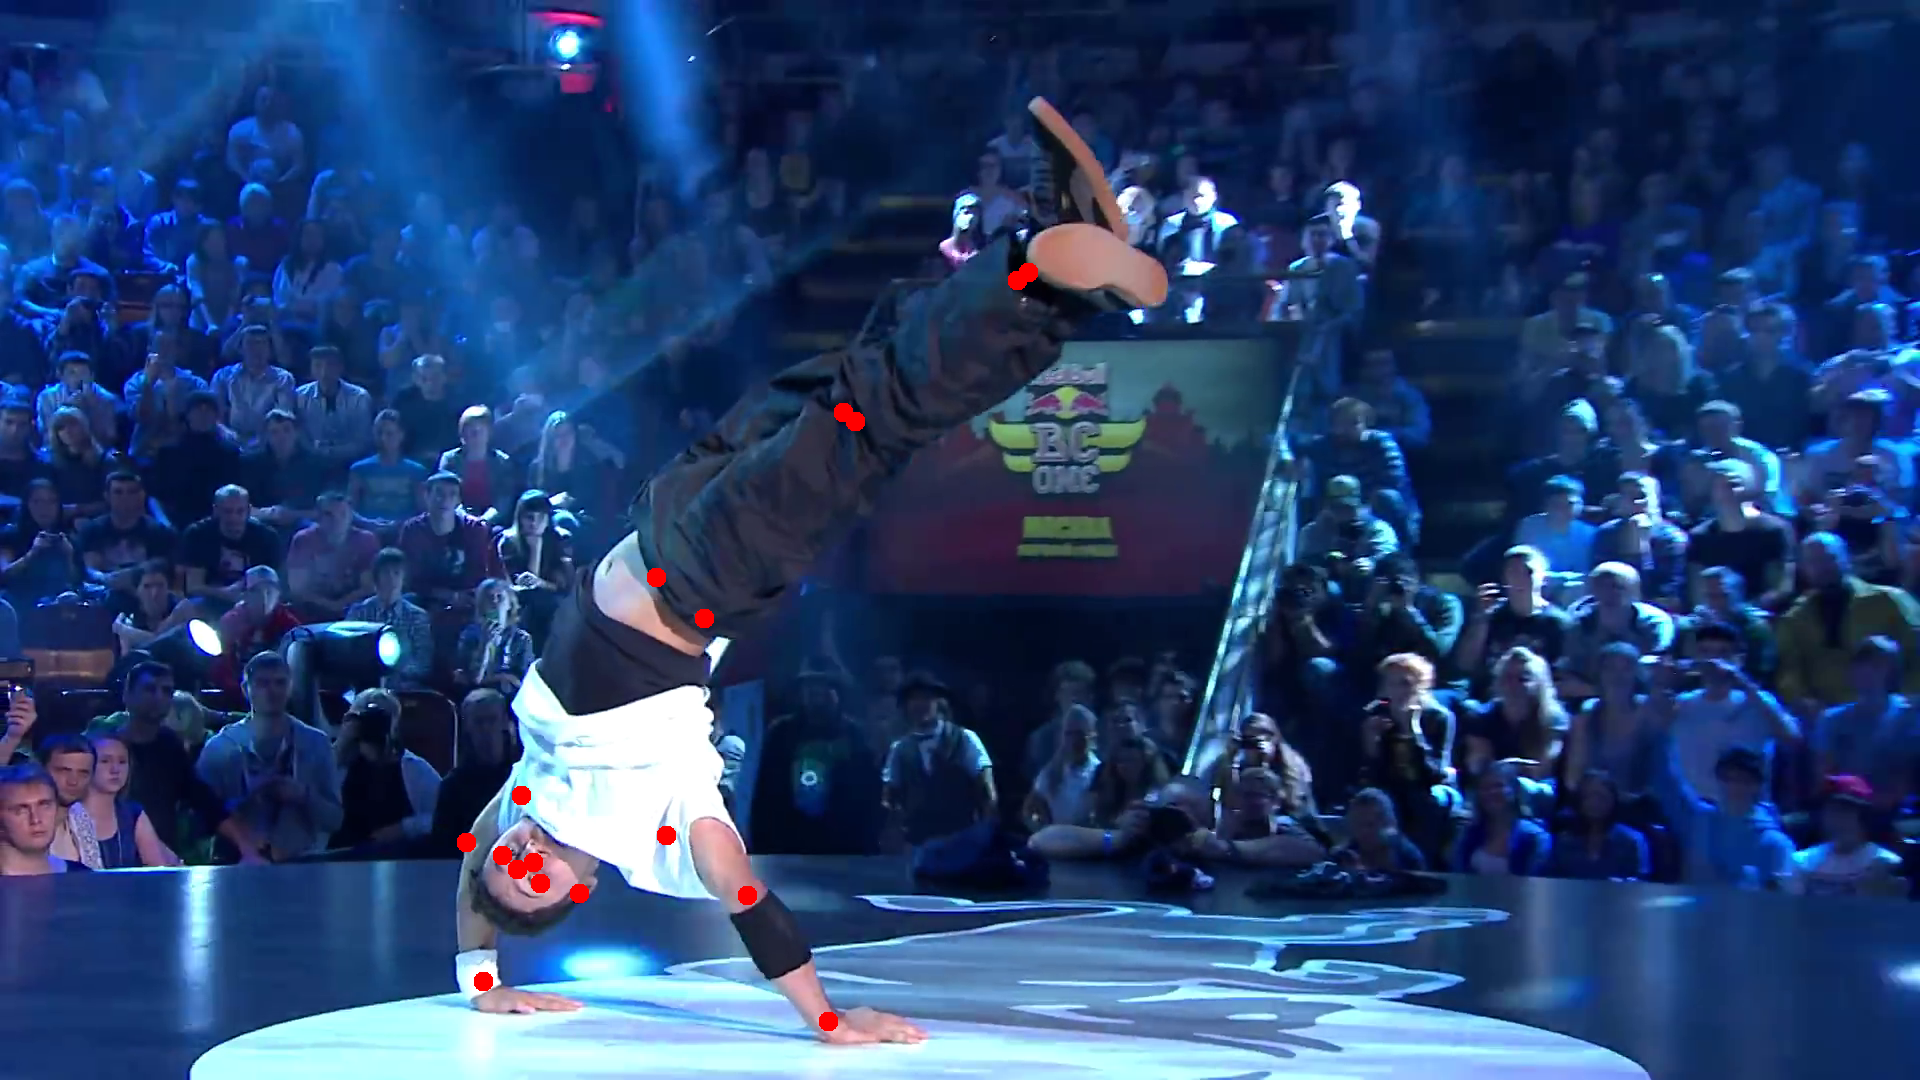
\includegraphics[width=\textwidth]{entities/BRACE_2454.png}
        \caption{Frame 2454}
    \end{subfigure}

    \caption{Example of five consecutive frames of a video from the BRACE dataset with the corresponding groundtruth keypoints,
    where the actor holds his position for a while.}
    \label{fig:BRACE_dataset_static}
\end{figure}

\begin{figure}[htbp]
    \centering
    \begin{subfigure}{0.45\textwidth}
        \centering
        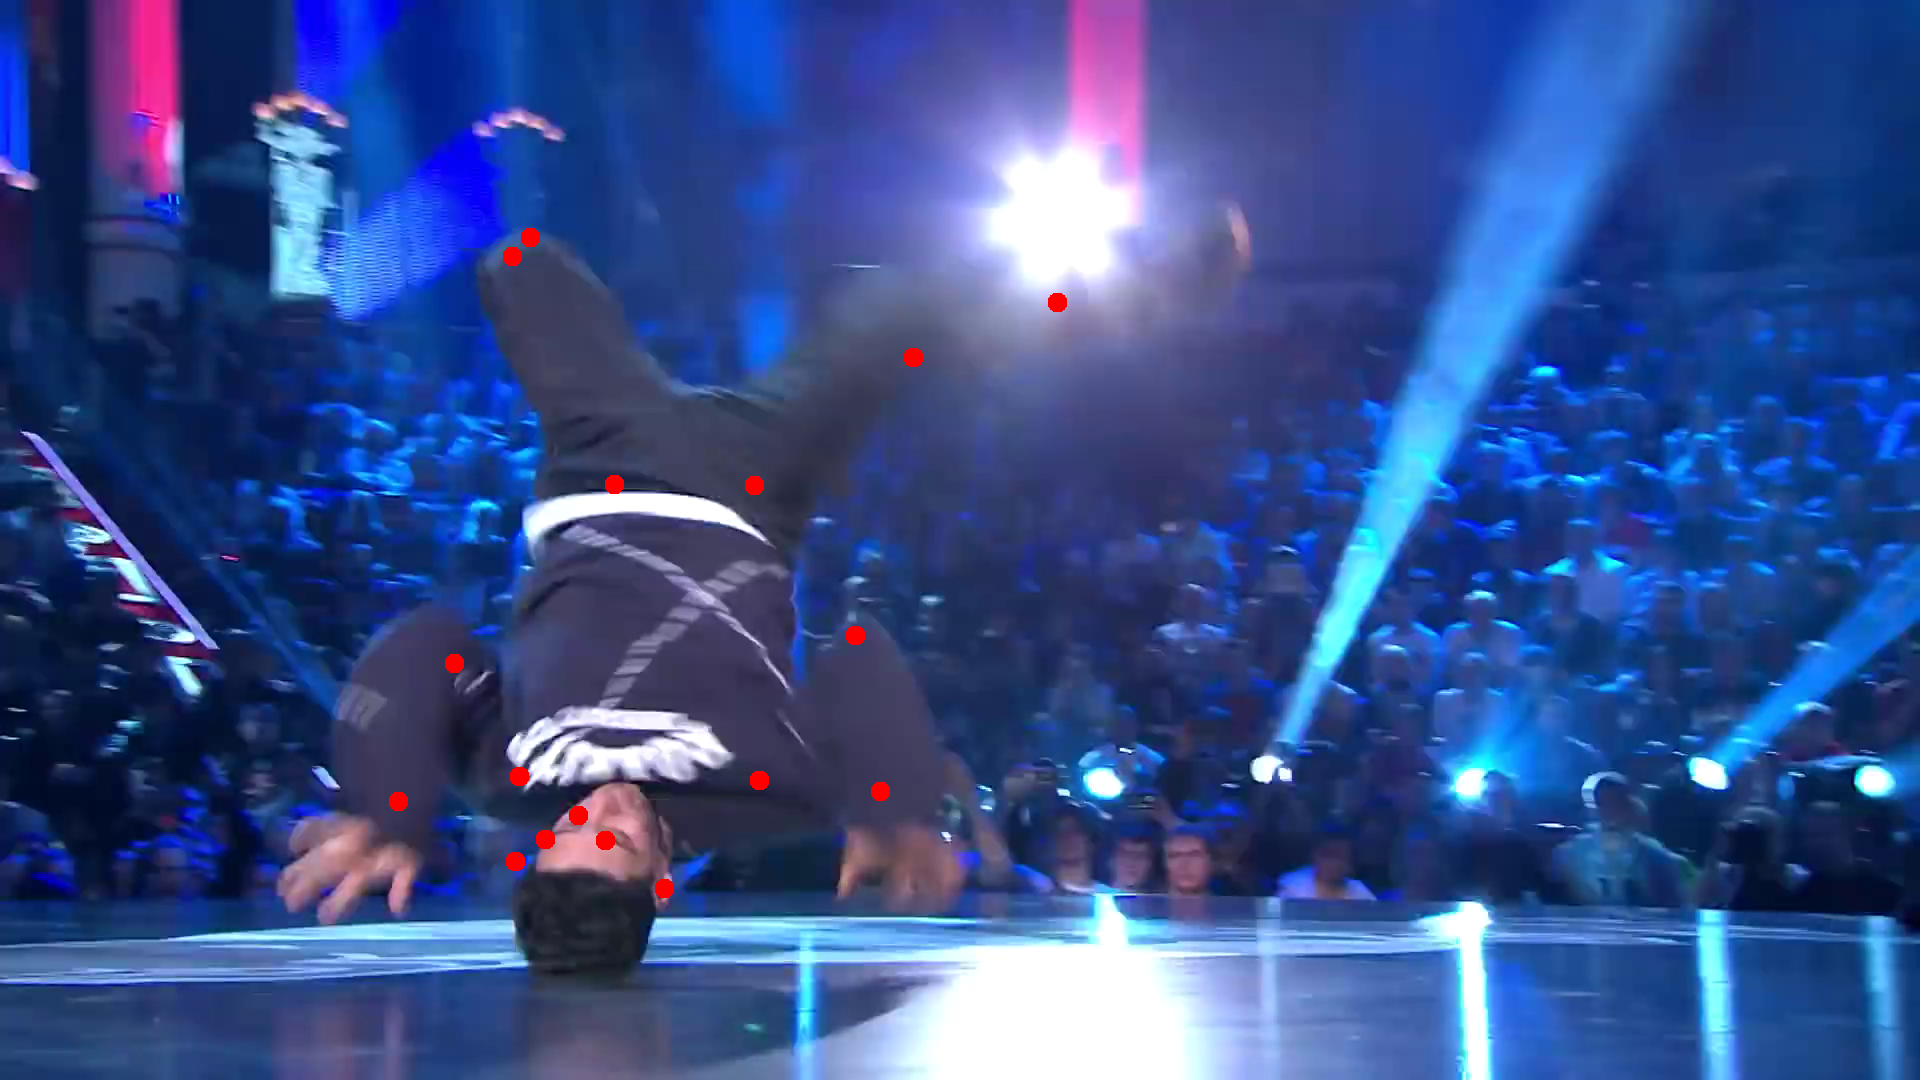
\includegraphics[width=\textwidth]{entities/BRACE_1148.png}
        \caption{Frame 1148}
    \end{subfigure}
    \begin{subfigure}{0.45\textwidth}
        \centering
        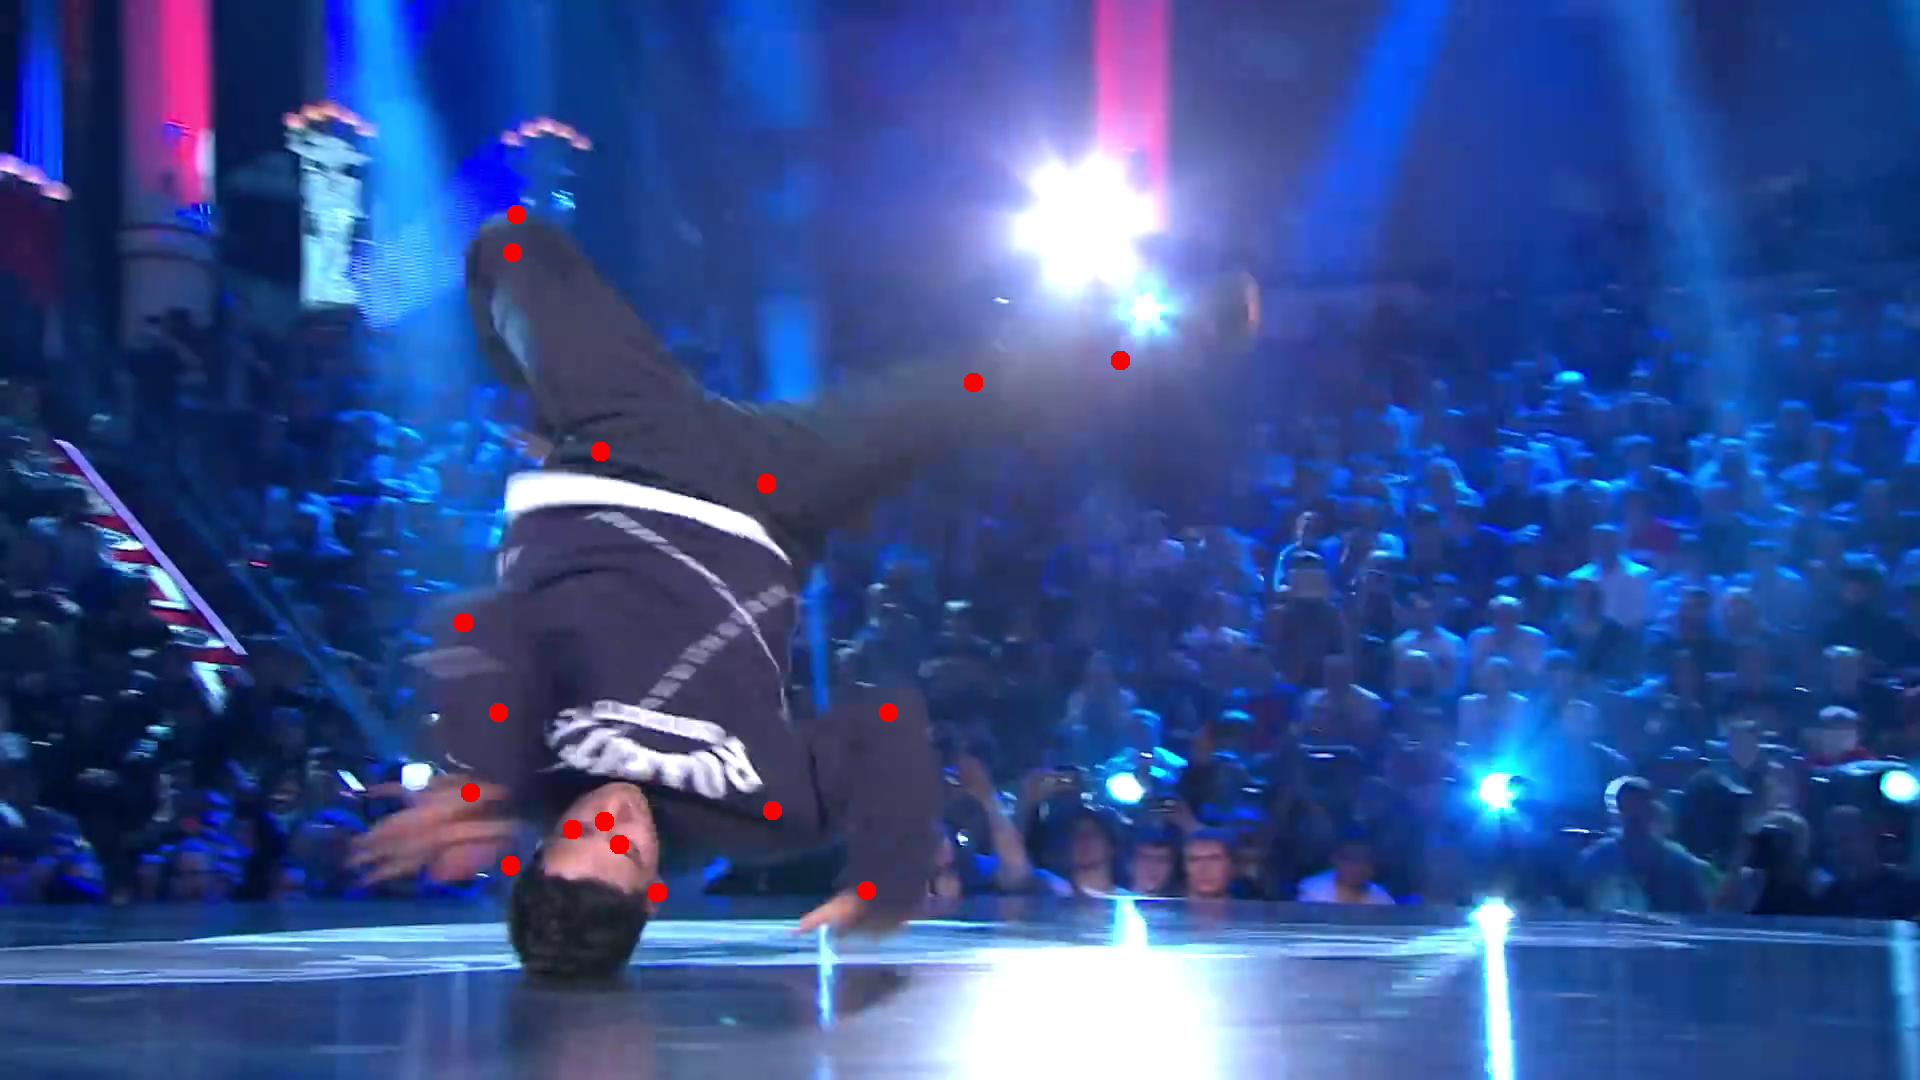
\includegraphics[width=\textwidth]{entities/BRACE_1149.png}
        \caption{Frame 1149}
    \end{subfigure}
    \begin{subfigure}{0.45\textwidth}
        \centering
        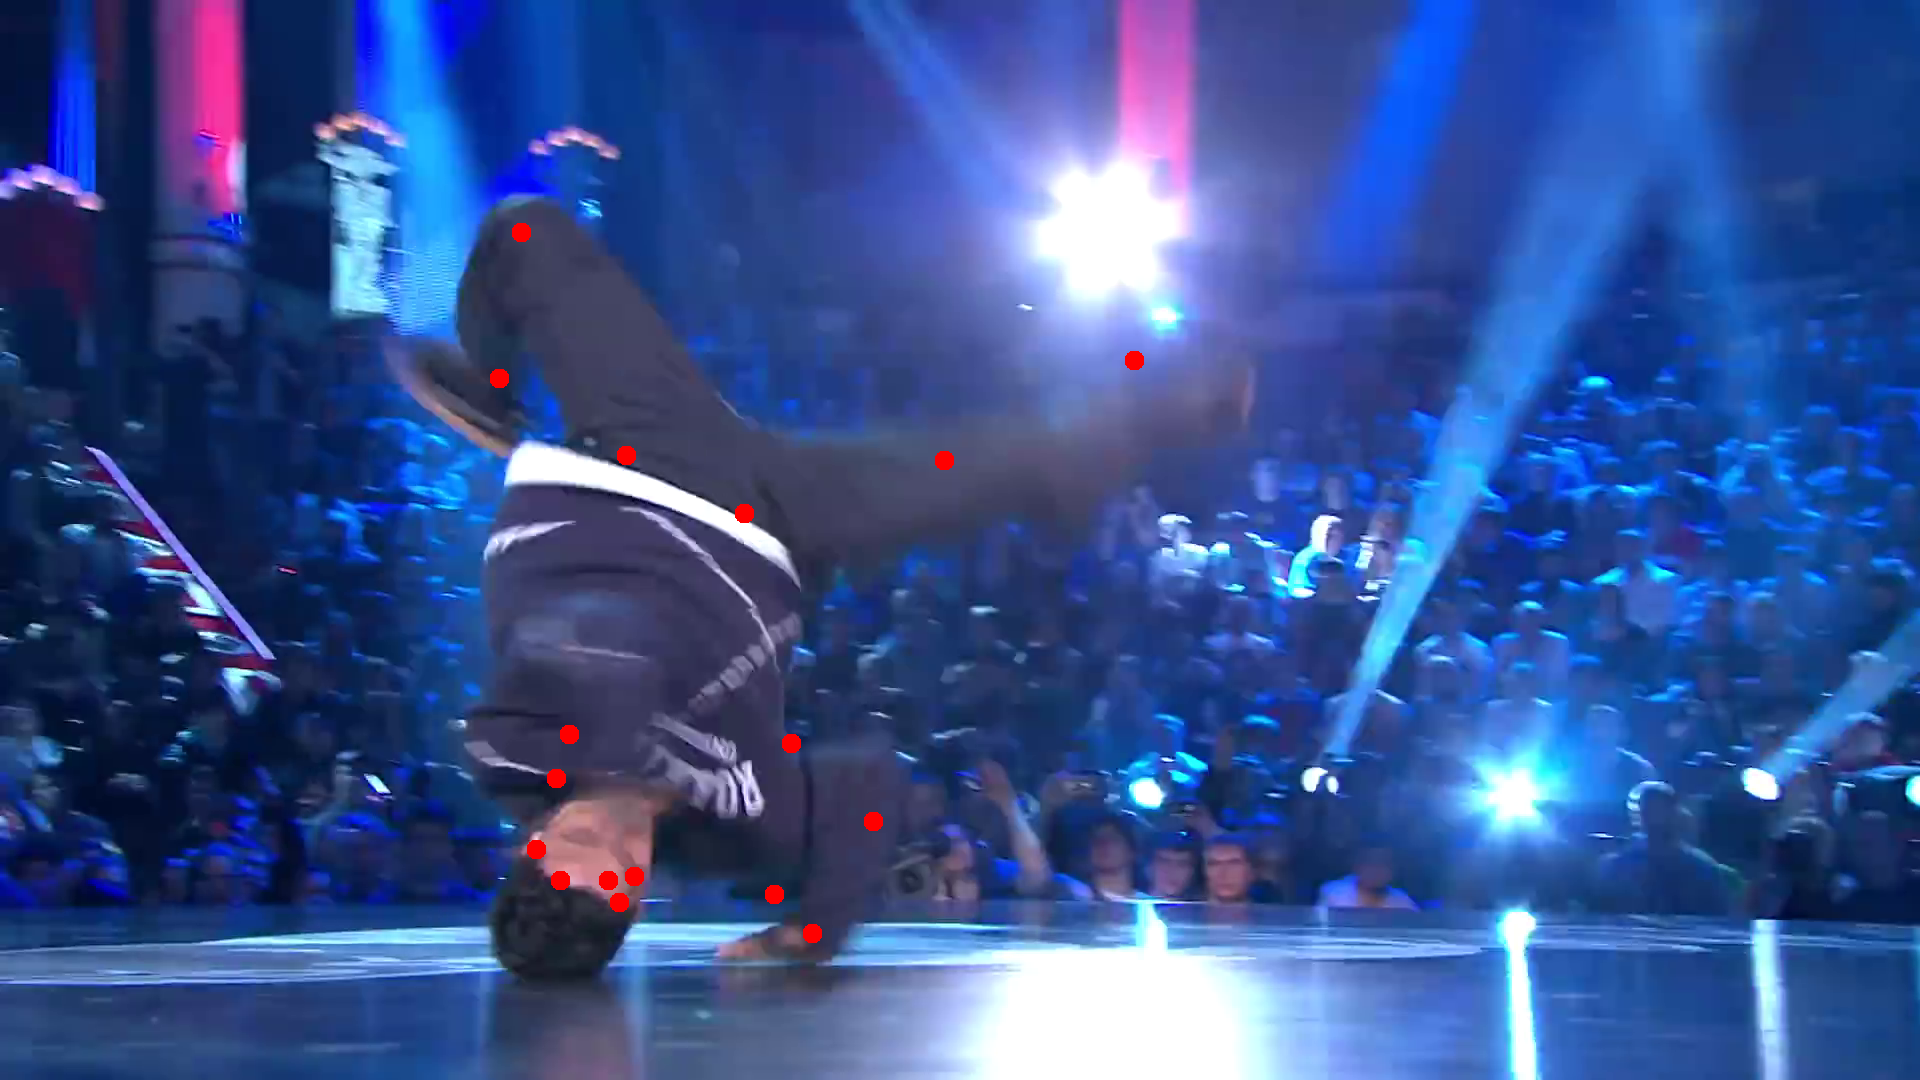
\includegraphics[width=\textwidth]{entities/BRACE_1150.png}
        \caption{Frame 1150}
    \end{subfigure}
    \begin{subfigure}{0.45\textwidth}
        \centering
        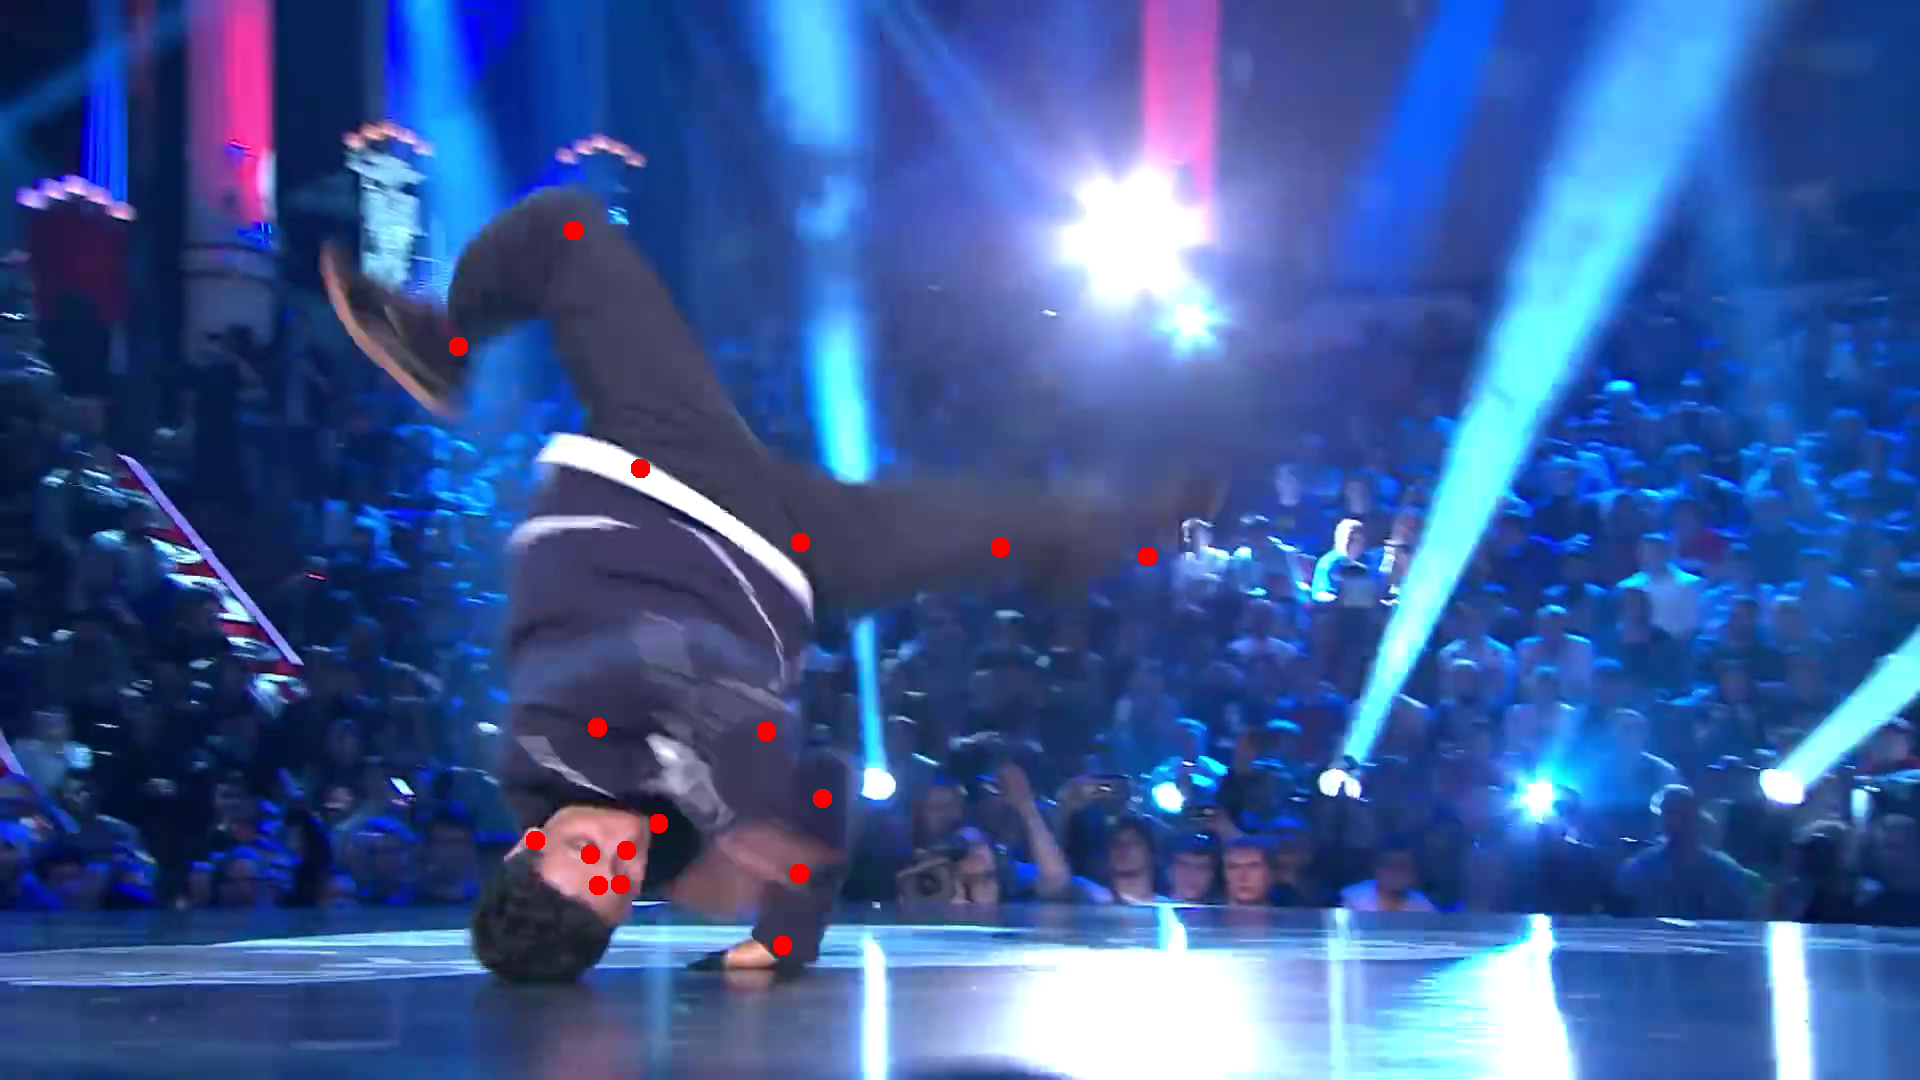
\includegraphics[width=\textwidth]{entities/BRACE_1151.png}
        \caption{Frame 1151}
    \end{subfigure}
    \begin{subfigure}{0.45\textwidth}
        \centering
        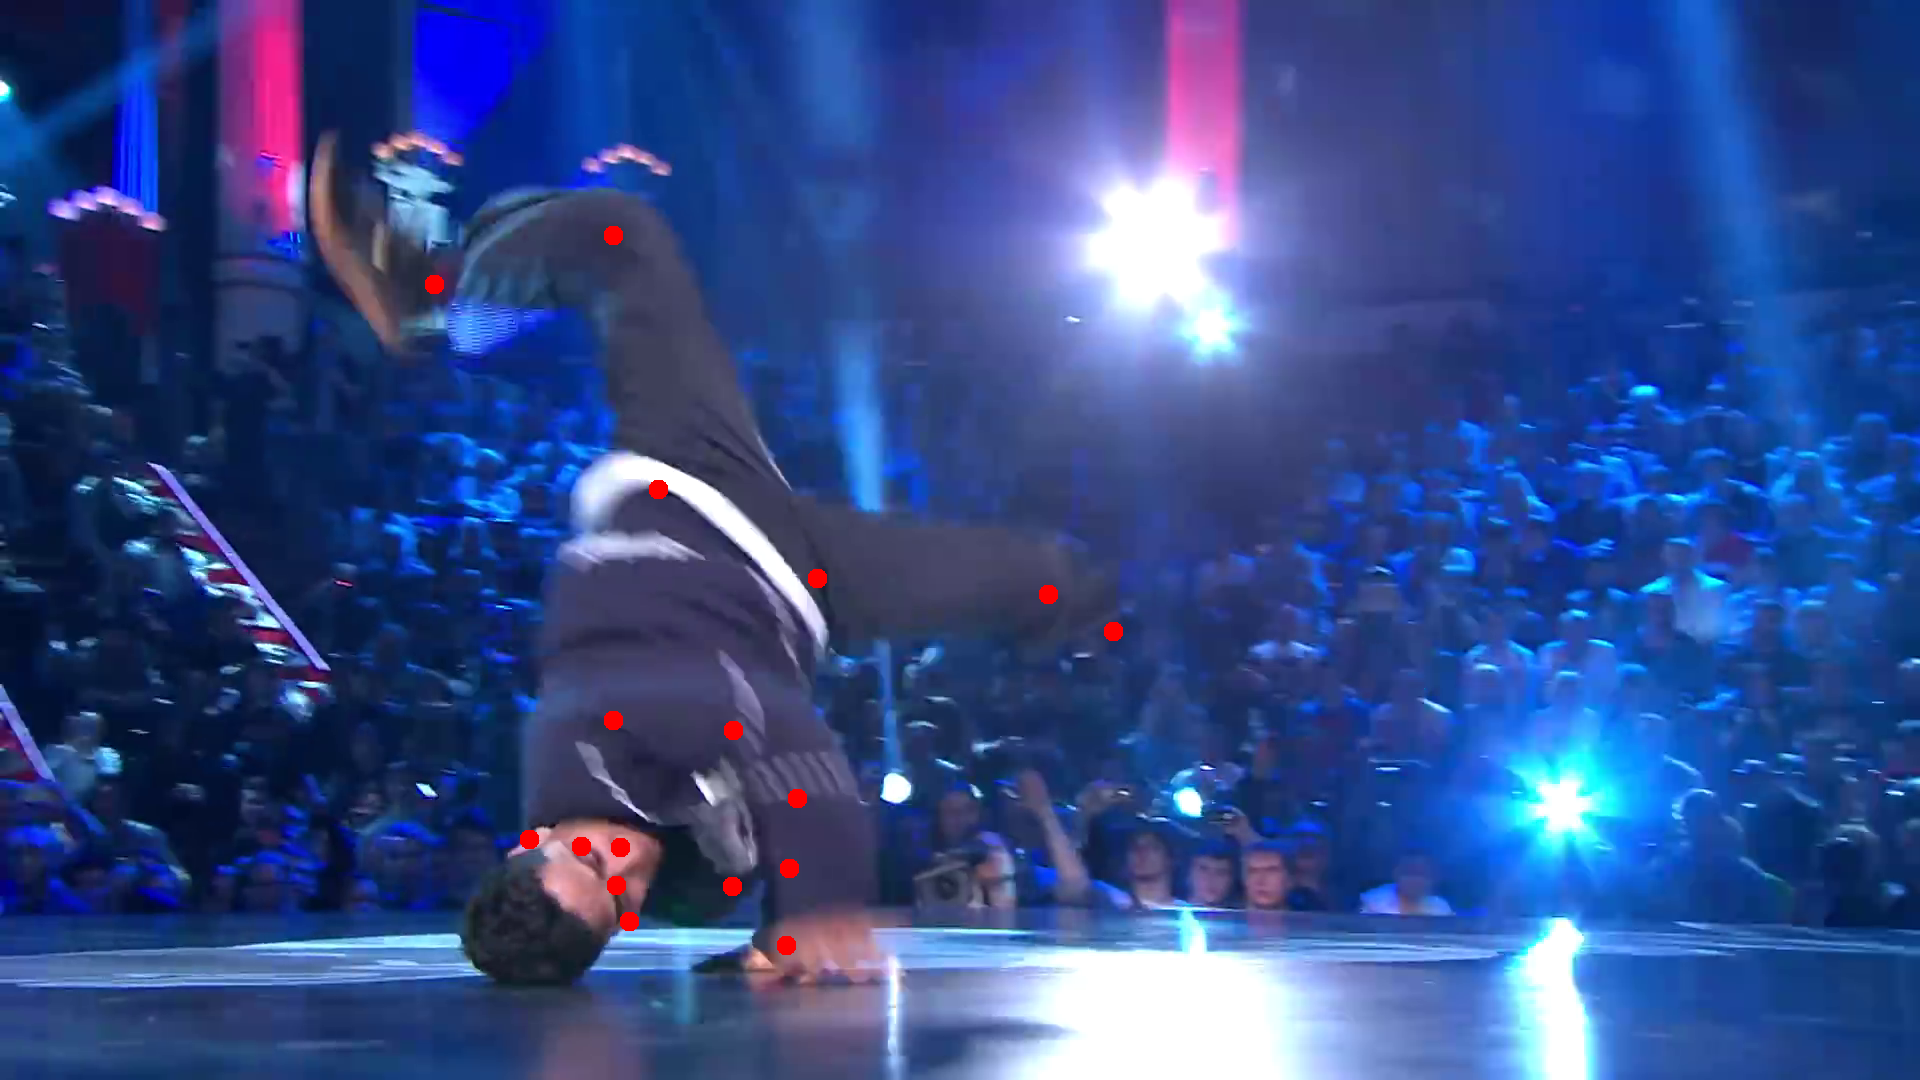
\includegraphics[width=\textwidth]{entities/BRACE_1152.png}
        \caption{Frame 1152}
    \end{subfigure}
    \caption{Example of five consecutive frames of a video from the BRACE dataset with the corresponding groundtruth keypoints, where the actor performs a quick movement.}
    \label{fig:BRACE_dataset_quick}
\end{figure}

\noindent The second dataset we will be using is the \textit{BRACE} dataset \cite{BRACE}. This dataset consists of $1,352$ video sequences and a total of $334,538$ frames with keypoints annotations of breakdancers. The frames of the video sequences have a resolution of $1920 \times 1080$ \cite{BRACE}.
\\
\\
We chose to use this dataset as breakdancers tend to swap between static and quick poses, as well as containing some acrobatic poses, similarly to the ones seen in the ClimbAlong dataset. Generally, the movements of the BRACE dataset are quicker than the movements of the ClimbAlong dataset. The static poses of the BRACE dataset tend to occur less frequently than the static poses of the the ClimbAlong dataset, as well as the quick movements tend to be quicker than the quick movements of the ClimbAlong dataset. However, as both the actors of both datasets swap between static and quick poses, as well as both datasets containing acrobatic poses, we found the BRACE dataset relevant for our experiments in Section \ref{sec:experiments}. Figure \ref{fig:BRACE_dataset_static} and \ref{fig:BRACE_dataset_quick} contains two consecutive sequences, each of five frames, that illustrates these two cases.
\\
\\
The frames of the video sequences have been annotated by initially using state-of-the-art human pose estimators to extract automatic poses. This was then followed by manually annotating bad keypoints, corresponding to difficult poses, as well as pose outliers. Finally, the automatic and manual annotations were merged by using interpolating. Each frame-annotation consists of $17$ keypoints, following the COCO-format, as illustrated in Table \ref{tab:keypoints} \cite{BRACE}.

\subsection{The Penn Action Dataset}
\label{sec:PA}
\begin{table}
    \begin{tabular}[htbp]{lllllllllllllll}
        \texttt{baseball\_pitch} & \texttt{baseball\_swing} & \texttt{bench\_press} \\
        \texttt{bowling} & \texttt{clean\_and\_jerk} & \texttt{golf\_swing} \\
        \texttt{jumping\_jacks} & \texttt{jump\_rope} & \texttt{pull\_ups} \\
        \texttt{push\_ups} & \texttt{sit\_ups} & \texttt{squats} \\
        \texttt{strumming\_guitar} & \texttt{tennis\_forehand} & \texttt{tennis\_serve}
    \end{tabular}
    \caption{The original $15$ action-types in the Penn Action dataset.}
    \label{tab:PA_actions}
\end{table}

\begin{figure}[htbp]
    \centering
    \begin{subfigure}{0.45\textwidth}
        \centering
        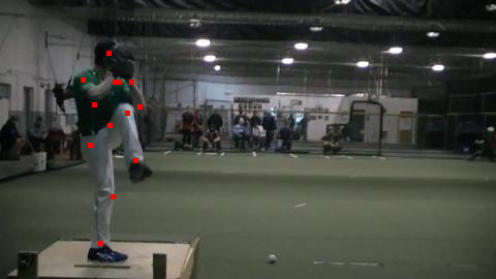
\includegraphics[width=\textwidth]{entities/PA_60.png}
        \caption{Frame 1148}
    \end{subfigure}
    \begin{subfigure}{0.45\textwidth}
        \centering
        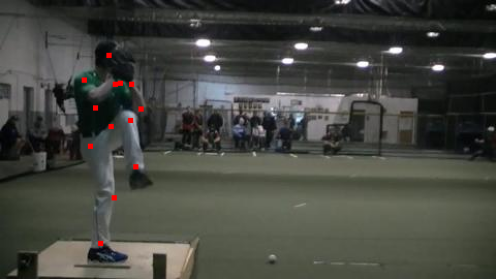
\includegraphics[width=\textwidth]{entities/PA_61.png}
        \caption{Frame 1149}
    \end{subfigure}
    \begin{subfigure}{0.45\textwidth}
        \centering
        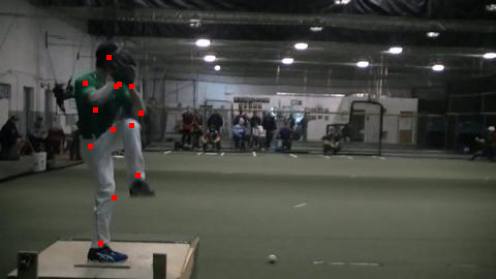
\includegraphics[width=\textwidth]{entities/PA_62.png}
        \caption{Frame 1150}
    \end{subfigure}
    \begin{subfigure}{0.45\textwidth}
        \centering
        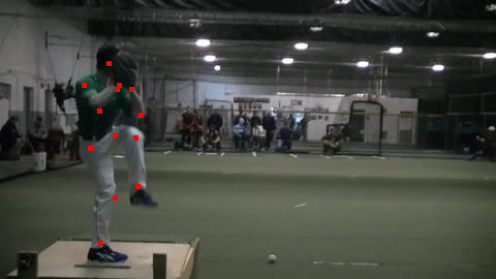
\includegraphics[width=\textwidth]{entities/PA_63.png}
        \caption{Frame 1151}
    \end{subfigure}
    \begin{subfigure}{0.45\textwidth}
        \centering
        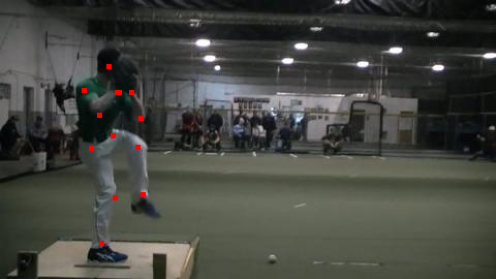
\includegraphics[width=\textwidth]{entities/PA_64.png}
        \caption{Frame 1152}
    \end{subfigure}
    \caption{Example of five consecutive frames of a video from the Penn Action dataset with the corresponding groundtruth keypoints.}
    \label{fig:PA_dataset}
\end{figure}
The final dataset we will be using is the \textit{Penn Action} dataset \cite{penn_action}. This dataset consists of $2,326$ video sequences of $15$ different action-types. Table \ref{tab:PA_actions} lists these $15$ action-types \cite{penn_action}. Each frame have a resolution within the size of $640 \times 480$ \cite{penn_action}.
\\
\\
Each sequence has been manually annotated with human joint annotation, consisting of $13$ joints as well as a corresponding binary visibility-flag for each joint. The placement of the invincible keypoints is very inconsistent, as some of the positions have been estimated, whereas others have been placed near one of the corners the image.
\\
\\
Unlike the BRACE dataset, most of the poses in the Penn Action dataset are not very unusual and thus are not very relevant for the poses of climbers. For that reason, we have decided to focus on the action-types that may contain more unusual poses. Thus, we only keep the sequences that have \texttt{baseball\_pitch}, \texttt{bench\_press} or \texttt{sit\_ups} as their corresponding action-type \cite{penn_action}. Further, the movements of the Penn Action dataset tend to be of a more similar pace to the ClimbAlong dataset than the BRACE dataset, making the Penn Action dataset relevant for our task.
\\
\\
In total, we use $307$ video sequences from the Penn Action dataset, consisting of a total of $26,036$ frames. Figure \ref{fig:PA_dataset} illustrates five consecutive frames with its groundtruth annotations for one of these video sequences.

\end{document}